% Created by tikzDevice version 0.12.6 on 2026-09-09 19:44:02
% !TEX encoding = UTF-8 Unicode
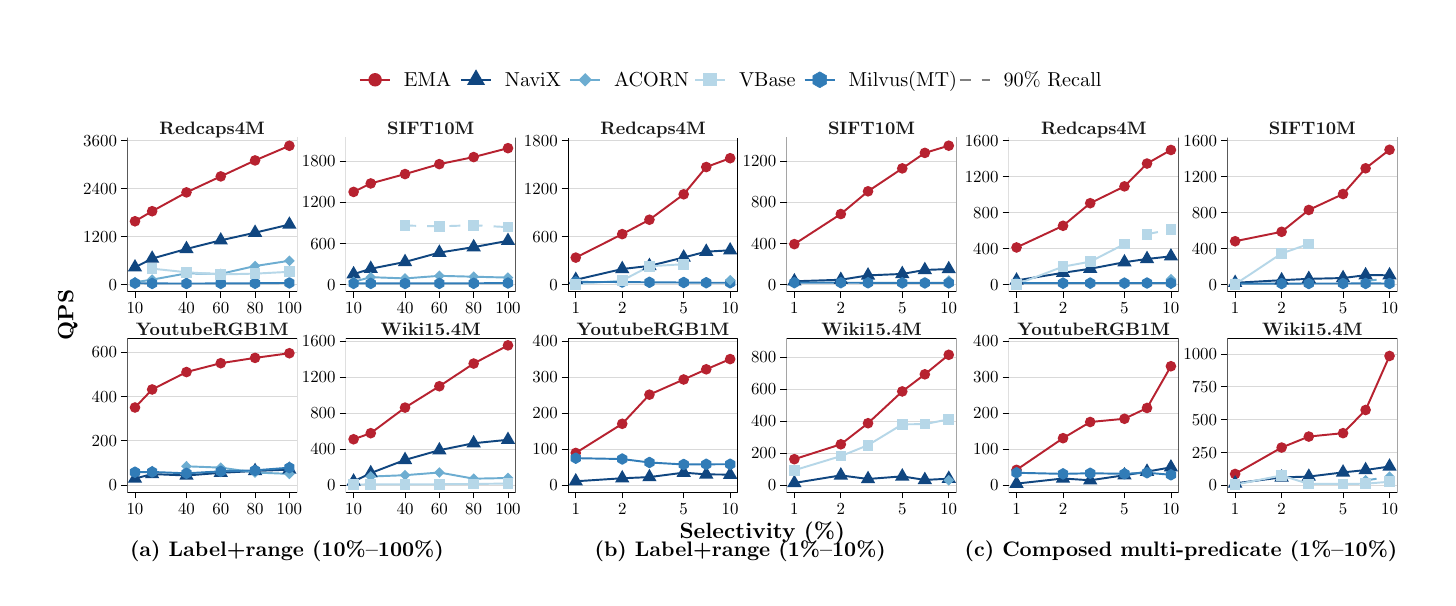
\begin{tikzpicture}[x=1pt,y=1pt]
\definecolor{fillColor}{RGB}{255,255,255}
\path[use as bounding box,fill=fillColor,fill opacity=0.00] (0,0) rectangle (505.89,198.74);
\begin{scope}
\path[clip] (  0.00,  0.00) rectangle (505.89,198.74);
\definecolor{drawColor}{RGB}{255,255,255}
\definecolor{fillColor}{RGB}{255,255,255}

\path[draw=drawColor,line width= 0.6pt,line join=round,line cap=round,fill=fillColor] (  0.00,  0.00) rectangle (505.89,198.74);
\end{scope}
\begin{scope}
\path[clip] (  5.50,165.59) rectangle (500.39,193.24);
\definecolor{drawColor}{RGB}{255,255,255}
\definecolor{fillColor}{RGB}{255,255,255}

\path[draw=drawColor,line width= 0.6pt,line join=round,line cap=round,fill=fillColor] (  5.50,165.59) rectangle (500.39,193.24);
\end{scope}
\begin{scope}
\path[clip] (  0.00,  0.00) rectangle (505.89,198.74);
\definecolor{fillColor}{RGB}{255,255,255}

\path[fill=fillColor] (118.71,174.93) rectangle (387.18,183.90);
\end{scope}
\begin{scope}
\path[clip] (  0.00,  0.00) rectangle (505.89,198.74);
\definecolor{drawColor}{RGB}{183,34,48}

\path[draw=drawColor,line width= 0.7pt,line join=round] (120.08,179.91) -- (131.01,179.91);
\definecolor{fillColor}{RGB}{183,34,48}

\path[fill=fillColor] (125.54,179.91) circle (  2.43);
\end{scope}
\begin{scope}
\path[clip] (  0.00,  0.00) rectangle (505.89,198.74);
\definecolor{drawColor}{RGB}{16,70,128}

\path[draw=drawColor,line width= 0.7pt,line join=round] (156.55,179.91) -- (167.47,179.91);
\definecolor{fillColor}{RGB}{16,70,128}

\path[fill=fillColor] (162.01,183.69) --
	(165.28,178.03) --
	(158.74,178.03) --
	cycle;
\end{scope}
\begin{scope}
\path[clip] (  0.00,  0.00) rectangle (505.89,198.74);
\definecolor{drawColor}{RGB}{109,173,209}

\path[draw=drawColor,line width= 0.7pt,line join=round] (196.00,179.91) -- (206.92,179.91);
\definecolor{fillColor}{RGB}{109,173,209}

\path[fill=fillColor] (199.03,179.91) --
	(201.46,182.34) --
	(203.89,179.91) --
	(201.46,177.49) --
	cycle;
\end{scope}
\begin{scope}
\path[clip] (  0.00,  0.00) rectangle (505.89,198.74);
\definecolor{drawColor}{RGB}{182,215,232}

\path[draw=drawColor,line width= 0.7pt,line join=round] (241.17,179.91) -- (252.09,179.91);
\definecolor{fillColor}{RGB}{182,215,232}

\path[fill=fillColor] (244.20,177.49) --
	(249.06,177.49) --
	(249.06,182.34) --
	(244.20,182.34) --
	cycle;
\end{scope}
\begin{scope}
\path[clip] (  0.00,  0.00) rectangle (505.89,198.74);
\definecolor{drawColor}{RGB}{49,124,183}

\path[draw=drawColor,line width= 0.7pt,line join=round] (280.76,179.91) -- (291.68,179.91);
\definecolor{fillColor}{RGB}{49,124,183}

\path[draw=drawColor,line width= 0.2pt,line join=round,line cap=round,fill=fillColor] (288.71,181.35) --
	(286.22,182.79) --
	(283.72,181.35) --
	(283.72,178.47) --
	(286.22,177.03) --
	(288.71,178.47) --
	(288.71,181.35) --
	cycle;
\end{scope}
\begin{scope}
\path[clip] (  0.00,  0.00) rectangle (505.89,198.74);
\definecolor{drawColor}{gray}{0.50}

\path[draw=drawColor,line width= 0.7pt,dash pattern=on 4pt off 4pt ,line join=round] (336.74,179.91) -- (347.67,179.91);
\end{scope}
\begin{scope}
\path[clip] (  0.00,  0.00) rectangle (505.89,198.74);
\definecolor{drawColor}{RGB}{0,0,0}

\node[text=drawColor,anchor=base west,inner sep=0pt, outer sep=0pt, scale=  0.73] at (135.97,177.40) {EMA};
\end{scope}
\begin{scope}
\path[clip] (  0.00,  0.00) rectangle (505.89,198.74);
\definecolor{drawColor}{RGB}{0,0,0}

\node[text=drawColor,anchor=base west,inner sep=0pt, outer sep=0pt, scale=  0.73] at (172.44,177.40) {NaviX};
\end{scope}
\begin{scope}
\path[clip] (  0.00,  0.00) rectangle (505.89,198.74);
\definecolor{drawColor}{RGB}{0,0,0}

\node[text=drawColor,anchor=base west,inner sep=0pt, outer sep=0pt, scale=  0.73] at (211.89,177.40) {ACORN};
\end{scope}
\begin{scope}
\path[clip] (  0.00,  0.00) rectangle (505.89,198.74);
\definecolor{drawColor}{RGB}{0,0,0}

\node[text=drawColor,anchor=base west,inner sep=0pt, outer sep=0pt, scale=  0.73] at (257.06,177.40) {VBase};
\end{scope}
\begin{scope}
\path[clip] (  0.00,  0.00) rectangle (505.89,198.74);
\definecolor{drawColor}{RGB}{0,0,0}

\node[text=drawColor,anchor=base west,inner sep=0pt, outer sep=0pt, scale=  0.73] at (296.65,177.40) {Milvus(MT)};
\end{scope}
\begin{scope}
\path[clip] (  0.00,  0.00) rectangle (505.89,198.74);
\definecolor{drawColor}{RGB}{0,0,0}

\node[text=drawColor,anchor=base west,inner sep=0pt, outer sep=0pt, scale=  0.73] at (352.64,177.40) {90\% Recall};
\end{scope}
\begin{scope}
\path[clip] (  5.50,  5.50) rectangle (177.85,165.59);
\definecolor{fillColor}{RGB}{255,255,255}

\path[fill=fillColor] (  5.50,  5.50) rectangle (177.85,165.59);
\end{scope}
\begin{scope}
\path[clip] (177.85,  5.50) rectangle (337.12,165.59);
\definecolor{fillColor}{RGB}{255,255,255}

\path[fill=fillColor] (177.85,  5.50) rectangle (337.12,165.59);
\end{scope}
\begin{scope}
\path[clip] (337.12,  5.50) rectangle (500.39,165.59);
\definecolor{fillColor}{RGB}{255,255,255}

\path[fill=fillColor] (337.12,  5.50) rectangle (500.39,165.59);
\end{scope}
\begin{scope}
\path[clip] ( 35.99,103.40) rectangle ( 97.36,159.04);
\definecolor{fillColor}{RGB}{255,255,255}

\path[fill=fillColor] ( 35.99,103.40) rectangle ( 97.36,159.04);
\definecolor{drawColor}{gray}{0.85}

\path[draw=drawColor,line width= 0.3pt,line join=round] ( 35.99,106.00) --
	( 97.36,106.00);

\path[draw=drawColor,line width= 0.3pt,line join=round] ( 35.99,123.33) --
	( 97.36,123.33);

\path[draw=drawColor,line width= 0.3pt,line join=round] ( 35.99,140.66) --
	( 97.36,140.66);

\path[draw=drawColor,line width= 0.3pt,line join=round] ( 35.99,158.00) --
	( 97.36,158.00);
\definecolor{drawColor}{RGB}{183,34,48}

\path[draw=drawColor,line width= 0.7pt,line join=round] ( 38.78,128.78) --
	( 44.98,132.42) --
	( 57.38,139.22) --
	( 69.77,145.00) --
	( 82.17,150.77) --
	( 94.57,156.06);
\definecolor{drawColor}{RGB}{16,70,128}

\path[draw=drawColor,line width= 0.7pt,line join=round] ( 38.78,112.14) --
	( 44.98,115.31) --
	( 57.38,118.78) --
	( 69.77,121.89) --
	( 82.17,124.66) --
	( 94.57,127.59);
\definecolor{drawColor}{RGB}{109,173,209}

\path[draw=drawColor,line width= 0.7pt,line join=round] ( 38.78,106.74) --
	( 44.98,107.70) --
	( 57.38,109.94) --
	( 69.77,109.78) --
	( 82.17,112.61) --
	( 94.57,114.51);
\definecolor{drawColor}{RGB}{49,124,183}

\path[draw=drawColor,line width= 0.7pt,line join=round] ( 38.78,106.43) --
	( 44.98,106.33) --
	( 57.38,106.28) --
	( 69.77,106.33) --
	( 82.17,106.38) --
	( 94.57,106.50);
\definecolor{drawColor}{RGB}{182,215,232}

\path[draw=drawColor,line width= 0.7pt,line join=round] ( 44.98,111.66) --
	( 57.38,110.36) --
	( 69.77,109.58) --
	( 82.17,109.86) --
	( 94.57,110.52);
\definecolor{fillColor}{RGB}{183,34,48}

\path[fill=fillColor] ( 94.57,156.06) circle (  1.93);

\path[fill=fillColor] ( 82.17,150.77) circle (  1.93);

\path[fill=fillColor] ( 69.77,145.00) circle (  1.93);

\path[fill=fillColor] ( 57.38,139.22) circle (  1.93);

\path[fill=fillColor] ( 44.98,132.42) circle (  1.93);

\path[fill=fillColor] ( 38.78,128.78) circle (  1.93);
\definecolor{fillColor}{RGB}{16,70,128}

\path[fill=fillColor] ( 94.57,130.59) --
	( 97.16,126.09) --
	( 91.97,126.09) --
	cycle;

\path[fill=fillColor] ( 82.17,127.66) --
	( 84.77,123.16) --
	( 79.57,123.16) --
	cycle;

\path[fill=fillColor] ( 69.77,124.88) --
	( 72.37,120.39) --
	( 67.18,120.39) --
	cycle;

\path[fill=fillColor] ( 57.38,121.78) --
	( 59.97,117.28) --
	( 54.78,117.28) --
	cycle;

\path[fill=fillColor] ( 44.98,118.31) --
	( 47.57,113.82) --
	( 42.38,113.82) --
	cycle;

\path[fill=fillColor] ( 38.78,115.14) --
	( 41.38,110.65) --
	( 36.18,110.65) --
	cycle;
\definecolor{fillColor}{RGB}{109,173,209}

\path[fill=fillColor] ( 92.64,114.51) --
	( 94.57,116.43) --
	( 96.50,114.51) --
	( 94.57,112.58) --
	cycle;

\path[fill=fillColor] ( 80.24,112.61) --
	( 82.17,114.54) --
	( 84.10,112.61) --
	( 82.17,110.68) --
	cycle;

\path[fill=fillColor] ( 67.85,109.78) --
	( 69.77,111.71) --
	( 71.70,109.78) --
	( 69.77,107.85) --
	cycle;

\path[fill=fillColor] ( 55.45,109.94) --
	( 57.38,111.87) --
	( 59.30,109.94) --
	( 57.38,108.01) --
	cycle;

\path[fill=fillColor] ( 43.05,107.70) --
	( 44.98,109.63) --
	( 46.91,107.70) --
	( 44.98,105.77) --
	cycle;

\path[fill=fillColor] ( 36.85,106.74) --
	( 38.78,108.66) --
	( 40.71,106.74) --
	( 38.78,104.81) --
	cycle;
\definecolor{drawColor}{RGB}{49,124,183}
\definecolor{fillColor}{RGB}{49,124,183}

\path[draw=drawColor,line width= 0.5pt,line join=round,line cap=round,fill=fillColor] ( 96.16,107.42) --
	( 94.57,108.33) --
	( 92.98,107.42) --
	( 92.98,105.58) --
	( 94.57,104.66) --
	( 96.16,105.58) --
	( 96.16,107.42) --
	cycle;
\end{scope}
\begin{scope}
\path[clip] ( 35.99,103.40) rectangle ( 97.36,159.04);
\definecolor{drawColor}{RGB}{49,124,183}
\definecolor{fillColor}{RGB}{49,124,183}

\path[draw=drawColor,line width= 0.5pt,line join=round,line cap=round,fill=fillColor] ( 83.76,107.30) --
	( 82.17,108.21) --
	( 80.58,107.30) --
	( 80.58,105.46) --
	( 82.17,104.54) --
	( 83.76,105.46) --
	( 83.76,107.30) --
	cycle;
\end{scope}
\begin{scope}
\path[clip] ( 35.99,103.40) rectangle ( 97.36,159.04);
\definecolor{drawColor}{RGB}{49,124,183}
\definecolor{fillColor}{RGB}{49,124,183}

\path[draw=drawColor,line width= 0.5pt,line join=round,line cap=round,fill=fillColor] ( 71.36,107.25) --
	( 69.77,108.17) --
	( 68.18,107.25) --
	( 68.18,105.41) --
	( 69.77,104.49) --
	( 71.36,105.41) --
	( 71.36,107.25) --
	cycle;
\end{scope}
\begin{scope}
\path[clip] ( 35.99,103.40) rectangle ( 97.36,159.04);
\definecolor{drawColor}{RGB}{49,124,183}
\definecolor{fillColor}{RGB}{49,124,183}

\path[draw=drawColor,line width= 0.5pt,line join=round,line cap=round,fill=fillColor] ( 58.97,107.20) --
	( 57.38,108.12) --
	( 55.78,107.20) --
	( 55.78,105.36) --
	( 57.38,104.45) --
	( 58.97,105.36) --
	( 58.97,107.20) --
	cycle;
\end{scope}
\begin{scope}
\path[clip] ( 35.99,103.40) rectangle ( 97.36,159.04);
\definecolor{drawColor}{RGB}{49,124,183}
\definecolor{fillColor}{RGB}{49,124,183}

\path[draw=drawColor,line width= 0.5pt,line join=round,line cap=round,fill=fillColor] ( 46.57,107.25) --
	( 44.98,108.16) --
	( 43.39,107.25) --
	( 43.39,105.41) --
	( 44.98,104.49) --
	( 46.57,105.41) --
	( 46.57,107.25) --
	cycle;
\end{scope}
\begin{scope}
\path[clip] ( 35.99,103.40) rectangle ( 97.36,159.04);
\definecolor{drawColor}{RGB}{49,124,183}
\definecolor{fillColor}{RGB}{49,124,183}

\path[draw=drawColor,line width= 0.5pt,line join=round,line cap=round,fill=fillColor] ( 40.37,107.35) --
	( 38.78,108.27) --
	( 37.19,107.35) --
	( 37.19,105.51) --
	( 38.78,104.59) --
	( 40.37,105.51) --
	( 40.37,107.35) --
	cycle;
\end{scope}
\begin{scope}
\path[clip] ( 35.99,103.40) rectangle ( 97.36,159.04);
\definecolor{fillColor}{RGB}{182,215,232}

\path[fill=fillColor] ( 92.64,108.59) --
	( 96.50,108.59) --
	( 96.50,112.45) --
	( 92.64,112.45) --
	cycle;

\path[fill=fillColor] ( 80.24,107.93) --
	( 84.10,107.93) --
	( 84.10,111.78) --
	( 80.24,111.78) --
	cycle;

\path[fill=fillColor] ( 67.85,107.65) --
	( 71.70,107.65) --
	( 71.70,111.50) --
	( 67.85,111.50) --
	cycle;

\path[fill=fillColor] ( 55.45,108.43) --
	( 59.30,108.43) --
	( 59.30,112.29) --
	( 55.45,112.29) --
	cycle;

\path[fill=fillColor] ( 43.05,109.73) --
	( 46.91,109.73) --
	( 46.91,113.58) --
	( 43.05,113.58) --
	cycle;
\definecolor{drawColor}{RGB}{0,0,0}

\path[draw=drawColor,line width= 0.4pt,line join=round,line cap=round] ( 35.99,103.40) rectangle ( 97.36,159.04);
\end{scope}
\begin{scope}
\path[clip] (114.98,103.40) rectangle (176.35,159.04);
\definecolor{fillColor}{RGB}{255,255,255}

\path[fill=fillColor] (114.98,103.40) rectangle (176.35,159.04);
\definecolor{drawColor}{gray}{0.85}

\path[draw=drawColor,line width= 0.3pt,line join=round] (114.98,106.00) --
	(176.35,106.00);

\path[draw=drawColor,line width= 0.3pt,line join=round] (114.98,120.85) --
	(176.35,120.85);

\path[draw=drawColor,line width= 0.3pt,line join=round] (114.98,135.71) --
	(176.35,135.71);

\path[draw=drawColor,line width= 0.3pt,line join=round] (114.98,150.57) --
	(176.35,150.57);
\definecolor{drawColor}{RGB}{183,34,48}

\path[draw=drawColor,line width= 0.7pt,line join=round] (117.77,139.39) --
	(123.97,142.45) --
	(136.36,145.84) --
	(148.76,149.43) --
	(161.16,151.98) --
	(173.56,155.20);
\definecolor{drawColor}{RGB}{16,70,128}

\path[draw=drawColor,line width= 0.7pt,line join=round] (117.77,109.67) --
	(123.97,111.63) --
	(136.36,114.08) --
	(148.76,117.46) --
	(161.16,119.44) --
	(173.56,121.72);
\definecolor{drawColor}{RGB}{109,173,209}

\path[draw=drawColor,line width= 0.7pt,line join=round] (117.77,106.90) --
	(123.97,108.59) --
	(136.36,108.13) --
	(148.76,109.07) --
	(161.16,108.75) --
	(173.56,108.43);
\definecolor{drawColor}{RGB}{49,124,183}

\path[draw=drawColor,line width= 0.7pt,line join=round] (117.77,106.34) --
	(123.97,106.33) --
	(136.36,106.31) --
	(148.76,106.34) --
	(161.16,106.37) --
	(173.56,106.46);
\definecolor{drawColor}{RGB}{182,215,232}

\path[draw=drawColor,line width= 0.7pt,dash pattern=on 4pt off 4pt ,line join=round] (136.36,127.24) --
	(148.76,126.95) --
	(161.16,127.35) --
	(173.56,126.65);
\definecolor{fillColor}{RGB}{183,34,48}

\path[fill=fillColor] (173.56,155.20) circle (  1.93);

\path[fill=fillColor] (161.16,151.98) circle (  1.93);

\path[fill=fillColor] (148.76,149.43) circle (  1.93);

\path[fill=fillColor] (136.36,145.84) circle (  1.93);

\path[fill=fillColor] (123.97,142.45) circle (  1.93);

\path[fill=fillColor] (117.77,139.39) circle (  1.93);
\definecolor{fillColor}{RGB}{16,70,128}

\path[fill=fillColor] (173.56,124.72) --
	(176.15,120.22) --
	(170.96,120.22) --
	cycle;

\path[fill=fillColor] (161.16,122.44) --
	(163.76,117.94) --
	(158.56,117.94) --
	cycle;

\path[fill=fillColor] (148.76,120.46) --
	(151.36,115.96) --
	(146.17,115.96) --
	cycle;

\path[fill=fillColor] (136.36,117.08) --
	(138.96,112.58) --
	(133.77,112.58) --
	cycle;

\path[fill=fillColor] (123.97,114.63) --
	(126.56,110.13) --
	(121.37,110.13) --
	cycle;

\path[fill=fillColor] (117.77,112.67) --
	(120.36,108.17) --
	(115.17,108.17) --
	cycle;
\definecolor{fillColor}{RGB}{109,173,209}

\path[fill=fillColor] (171.63,108.43) --
	(173.56,110.36) --
	(175.49,108.43) --
	(173.56,106.50) --
	cycle;

\path[fill=fillColor] (159.23,108.75) --
	(161.16,110.68) --
	(163.09,108.75) --
	(161.16,106.82) --
	cycle;

\path[fill=fillColor] (146.83,109.07) --
	(148.76,111.00) --
	(150.69,109.07) --
	(148.76,107.14) --
	cycle;

\path[fill=fillColor] (134.44,108.13) --
	(136.36,110.06) --
	(138.29,108.13) --
	(136.36,106.21) --
	cycle;

\path[fill=fillColor] (122.04,108.59) --
	(123.97,110.51) --
	(125.89,108.59) --
	(123.97,106.66) --
	cycle;

\path[fill=fillColor] (115.84,106.90) --
	(117.77,108.83) --
	(119.70,106.90) --
	(117.77,104.97) --
	cycle;
\definecolor{fillColor}{RGB}{182,215,232}

\path[fill=fillColor] (171.63,124.73) --
	(175.49,124.73) --
	(175.49,128.58) --
	(171.63,128.58) --
	cycle;

\path[fill=fillColor] (159.23,125.42) --
	(163.09,125.42) --
	(163.09,129.27) --
	(159.23,129.27) --
	cycle;

\path[fill=fillColor] (146.83,125.02) --
	(150.69,125.02) --
	(150.69,128.88) --
	(146.83,128.88) --
	cycle;

\path[fill=fillColor] (134.44,125.32) --
	(138.29,125.32) --
	(138.29,129.17) --
	(134.44,129.17) --
	cycle;
\definecolor{drawColor}{RGB}{49,124,183}
\definecolor{fillColor}{RGB}{49,124,183}

\path[draw=drawColor,line width= 0.5pt,line join=round,line cap=round,fill=fillColor] (175.15,107.38) --
	(173.56,108.30) --
	(171.97,107.38) --
	(171.97,105.54) --
	(173.56,104.62) --
	(175.15,105.54) --
	(175.15,107.38) --
	cycle;
\end{scope}
\begin{scope}
\path[clip] (114.98,103.40) rectangle (176.35,159.04);
\definecolor{drawColor}{RGB}{49,124,183}
\definecolor{fillColor}{RGB}{49,124,183}

\path[draw=drawColor,line width= 0.5pt,line join=round,line cap=round,fill=fillColor] (162.75,107.29) --
	(161.16,108.21) --
	(159.57,107.29) --
	(159.57,105.45) --
	(161.16,104.53) --
	(162.75,105.45) --
	(162.75,107.29) --
	cycle;
\end{scope}
\begin{scope}
\path[clip] (114.98,103.40) rectangle (176.35,159.04);
\definecolor{drawColor}{RGB}{49,124,183}
\definecolor{fillColor}{RGB}{49,124,183}

\path[draw=drawColor,line width= 0.5pt,line join=round,line cap=round,fill=fillColor] (150.35,107.26) --
	(148.76,108.17) --
	(147.17,107.26) --
	(147.17,105.42) --
	(148.76,104.50) --
	(150.35,105.42) --
	(150.35,107.26) --
	cycle;
\end{scope}
\begin{scope}
\path[clip] (114.98,103.40) rectangle (176.35,159.04);
\definecolor{drawColor}{RGB}{49,124,183}
\definecolor{fillColor}{RGB}{49,124,183}

\path[draw=drawColor,line width= 0.5pt,line join=round,line cap=round,fill=fillColor] (137.96,107.23) --
	(136.36,108.15) --
	(134.77,107.23) --
	(134.77,105.39) --
	(136.36,104.47) --
	(137.96,105.39) --
	(137.96,107.23) --
	cycle;
\end{scope}
\begin{scope}
\path[clip] (114.98,103.40) rectangle (176.35,159.04);
\definecolor{drawColor}{RGB}{49,124,183}
\definecolor{fillColor}{RGB}{49,124,183}

\path[draw=drawColor,line width= 0.5pt,line join=round,line cap=round,fill=fillColor] (125.56,107.25) --
	(123.97,108.17) --
	(122.38,107.25) --
	(122.38,105.41) --
	(123.97,104.50) --
	(125.56,105.41) --
	(125.56,107.25) --
	cycle;
\end{scope}
\begin{scope}
\path[clip] (114.98,103.40) rectangle (176.35,159.04);
\definecolor{drawColor}{RGB}{49,124,183}
\definecolor{fillColor}{RGB}{49,124,183}

\path[draw=drawColor,line width= 0.5pt,line join=round,line cap=round,fill=fillColor] (119.36,107.26) --
	(117.77,108.18) --
	(116.18,107.26) --
	(116.18,105.43) --
	(117.77,104.51) --
	(119.36,105.43) --
	(119.36,107.26) --
	cycle;
\end{scope}
\begin{scope}
\path[clip] (114.98,103.40) rectangle (176.35,159.04);
\definecolor{drawColor}{RGB}{0,0,0}

\path[draw=drawColor,line width= 0.4pt,line join=round,line cap=round] (114.98,103.40) rectangle (176.35,159.04);
\end{scope}
\begin{scope}
\path[clip] ( 35.99, 30.90) rectangle ( 97.36, 86.54);
\definecolor{fillColor}{RGB}{255,255,255}

\path[fill=fillColor] ( 35.99, 30.90) rectangle ( 97.36, 86.54);
\definecolor{drawColor}{gray}{0.85}

\path[draw=drawColor,line width= 0.3pt,line join=round] ( 35.99, 33.50) --
	( 97.36, 33.50);

\path[draw=drawColor,line width= 0.3pt,line join=round] ( 35.99, 49.50) --
	( 97.36, 49.50);

\path[draw=drawColor,line width= 0.3pt,line join=round] ( 35.99, 65.50) --
	( 97.36, 65.50);

\path[draw=drawColor,line width= 0.3pt,line join=round] ( 35.99, 81.50) --
	( 97.36, 81.50);
\definecolor{drawColor}{RGB}{183,34,48}

\path[draw=drawColor,line width= 0.7pt,line join=round] ( 38.78, 61.49) --
	( 44.98, 68.01) --
	( 57.38, 74.30) --
	( 69.77, 77.50) --
	( 82.17, 79.42) --
	( 94.57, 81.10);
\definecolor{drawColor}{RGB}{16,70,128}

\path[draw=drawColor,line width= 0.7pt,line join=round] ( 38.78, 35.80) --
	( 44.98, 37.44) --
	( 57.38, 36.92) --
	( 69.77, 37.89) --
	( 82.17, 38.55) --
	( 94.57, 39.04);
\definecolor{drawColor}{RGB}{109,173,209}

\path[draw=drawColor,line width= 0.7pt,line join=round] ( 57.38, 40.24) --
	( 69.77, 39.77) --
	( 82.17, 37.99) --
	( 94.57, 37.50);
\definecolor{drawColor}{RGB}{49,124,183}

\path[draw=drawColor,line width= 0.7pt,line join=round] ( 38.78, 38.11) --
	( 44.98, 38.20) --
	( 57.38, 37.71) --
	( 69.77, 38.42) --
	( 82.17, 38.79) --
	( 94.57, 39.74);
\definecolor{fillColor}{RGB}{183,34,48}

\path[fill=fillColor] ( 94.57, 81.10) circle (  1.93);

\path[fill=fillColor] ( 82.17, 79.42) circle (  1.93);

\path[fill=fillColor] ( 69.77, 77.50) circle (  1.93);

\path[fill=fillColor] ( 57.38, 74.30) circle (  1.93);

\path[fill=fillColor] ( 44.98, 68.01) circle (  1.93);

\path[fill=fillColor] ( 38.78, 61.49) circle (  1.93);
\definecolor{fillColor}{RGB}{16,70,128}

\path[fill=fillColor] ( 94.57, 42.04) --
	( 97.16, 37.55) --
	( 91.97, 37.55) --
	cycle;

\path[fill=fillColor] ( 82.17, 41.55) --
	( 84.77, 37.05) --
	( 79.57, 37.05) --
	cycle;

\path[fill=fillColor] ( 69.77, 40.89) --
	( 72.37, 36.39) --
	( 67.18, 36.39) --
	cycle;

\path[fill=fillColor] ( 57.38, 39.92) --
	( 59.97, 35.42) --
	( 54.78, 35.42) --
	cycle;

\path[fill=fillColor] ( 44.98, 40.43) --
	( 47.57, 35.94) --
	( 42.38, 35.94) --
	cycle;

\path[fill=fillColor] ( 38.78, 38.80) --
	( 41.38, 34.30) --
	( 36.18, 34.30) --
	cycle;
\definecolor{fillColor}{RGB}{109,173,209}

\path[fill=fillColor] ( 92.64, 37.50) --
	( 94.57, 39.42) --
	( 96.50, 37.50) --
	( 94.57, 35.57) --
	cycle;

\path[fill=fillColor] ( 80.24, 37.99) --
	( 82.17, 39.92) --
	( 84.10, 37.99) --
	( 82.17, 36.07) --
	cycle;

\path[fill=fillColor] ( 67.85, 39.77) --
	( 69.77, 41.70) --
	( 71.70, 39.77) --
	( 69.77, 37.84) --
	cycle;

\path[fill=fillColor] ( 55.45, 40.24) --
	( 57.38, 42.17) --
	( 59.30, 40.24) --
	( 57.38, 38.32) --
	cycle;
\definecolor{fillColor}{RGB}{49,124,183}

\path[draw=drawColor,line width= 0.5pt,line join=round,line cap=round,fill=fillColor] ( 96.16, 40.66) --
	( 94.57, 41.57) --
	( 92.98, 40.66) --
	( 92.98, 38.82) --
	( 94.57, 37.90) --
	( 96.16, 38.82) --
	( 96.16, 40.66) --
	cycle;
\end{scope}
\begin{scope}
\path[clip] ( 35.99, 30.90) rectangle ( 97.36, 86.54);
\definecolor{drawColor}{RGB}{49,124,183}
\definecolor{fillColor}{RGB}{49,124,183}

\path[draw=drawColor,line width= 0.5pt,line join=round,line cap=round,fill=fillColor] ( 83.76, 39.70) --
	( 82.17, 40.62) --
	( 80.58, 39.70) --
	( 80.58, 37.87) --
	( 82.17, 36.95) --
	( 83.76, 37.87) --
	( 83.76, 39.70) --
	cycle;
\end{scope}
\begin{scope}
\path[clip] ( 35.99, 30.90) rectangle ( 97.36, 86.54);
\definecolor{drawColor}{RGB}{49,124,183}
\definecolor{fillColor}{RGB}{49,124,183}

\path[draw=drawColor,line width= 0.5pt,line join=round,line cap=round,fill=fillColor] ( 71.36, 39.34) --
	( 69.77, 40.25) --
	( 68.18, 39.34) --
	( 68.18, 37.50) --
	( 69.77, 36.58) --
	( 71.36, 37.50) --
	( 71.36, 39.34) --
	cycle;
\end{scope}
\begin{scope}
\path[clip] ( 35.99, 30.90) rectangle ( 97.36, 86.54);
\definecolor{drawColor}{RGB}{49,124,183}
\definecolor{fillColor}{RGB}{49,124,183}

\path[draw=drawColor,line width= 0.5pt,line join=round,line cap=round,fill=fillColor] ( 58.97, 38.63) --
	( 57.38, 39.55) --
	( 55.78, 38.63) --
	( 55.78, 36.80) --
	( 57.38, 35.88) --
	( 58.97, 36.80) --
	( 58.97, 38.63) --
	cycle;
\end{scope}
\begin{scope}
\path[clip] ( 35.99, 30.90) rectangle ( 97.36, 86.54);
\definecolor{drawColor}{RGB}{49,124,183}
\definecolor{fillColor}{RGB}{49,124,183}

\path[draw=drawColor,line width= 0.5pt,line join=round,line cap=round,fill=fillColor] ( 46.57, 39.12) --
	( 44.98, 40.04) --
	( 43.39, 39.12) --
	( 43.39, 37.28) --
	( 44.98, 36.36) --
	( 46.57, 37.28) --
	( 46.57, 39.12) --
	cycle;
\end{scope}
\begin{scope}
\path[clip] ( 35.99, 30.90) rectangle ( 97.36, 86.54);
\definecolor{drawColor}{RGB}{49,124,183}
\definecolor{fillColor}{RGB}{49,124,183}

\path[draw=drawColor,line width= 0.5pt,line join=round,line cap=round,fill=fillColor] ( 40.37, 39.03) --
	( 38.78, 39.95) --
	( 37.19, 39.03) --
	( 37.19, 37.19) --
	( 38.78, 36.27) --
	( 40.37, 37.19) --
	( 40.37, 39.03) --
	cycle;
\end{scope}
\begin{scope}
\path[clip] ( 35.99, 30.90) rectangle ( 97.36, 86.54);
\definecolor{drawColor}{RGB}{0,0,0}

\path[draw=drawColor,line width= 0.4pt,line join=round,line cap=round] ( 35.99, 30.90) rectangle ( 97.36, 86.54);
\end{scope}
\begin{scope}
\path[clip] (114.98, 30.90) rectangle (176.35, 86.54);
\definecolor{fillColor}{RGB}{255,255,255}

\path[fill=fillColor] (114.98, 30.90) rectangle (176.35, 86.54);
\definecolor{drawColor}{gray}{0.85}

\path[draw=drawColor,line width= 0.3pt,line join=round] (114.98, 33.50) --
	(176.35, 33.50);

\path[draw=drawColor,line width= 0.3pt,line join=round] (114.98, 46.50) --
	(176.35, 46.50);

\path[draw=drawColor,line width= 0.3pt,line join=round] (114.98, 59.50) --
	(176.35, 59.50);

\path[draw=drawColor,line width= 0.3pt,line join=round] (114.98, 72.50) --
	(176.35, 72.50);

\path[draw=drawColor,line width= 0.3pt,line join=round] (114.98, 85.50) --
	(176.35, 85.50);
\definecolor{drawColor}{RGB}{183,34,48}

\path[draw=drawColor,line width= 0.7pt,line join=round] (117.77, 50.01) --
	(123.97, 52.21) --
	(136.36, 61.45) --
	(148.76, 69.17) --
	(161.16, 77.37) --
	(173.56, 83.94);
\definecolor{drawColor}{RGB}{16,70,128}

\path[draw=drawColor,line width= 0.7pt,line join=round] (117.77, 34.77) --
	(123.97, 37.79) --
	(136.36, 42.55) --
	(148.76, 46.06) --
	(161.16, 48.58) --
	(173.56, 49.82);
\definecolor{drawColor}{RGB}{109,173,209}

\path[draw=drawColor,line width= 0.7pt,line join=round] (123.97, 36.54) --
	(136.36, 37.03) --
	(148.76, 38.00) --
	(161.16, 35.77) --
	(173.56, 36.01);
\definecolor{drawColor}{RGB}{182,215,232}

\path[draw=drawColor,line width= 0.7pt,line join=round] (117.77, 33.58) --
	(123.97, 33.74) --
	(136.36, 33.67) --
	(148.76, 33.75) --
	(161.16, 33.86) --
	(173.56, 34.01);
\definecolor{fillColor}{RGB}{183,34,48}

\path[fill=fillColor] (173.56, 83.94) circle (  1.93);

\path[fill=fillColor] (161.16, 77.37) circle (  1.93);

\path[fill=fillColor] (148.76, 69.17) circle (  1.93);

\path[fill=fillColor] (136.36, 61.45) circle (  1.93);

\path[fill=fillColor] (123.97, 52.21) circle (  1.93);

\path[fill=fillColor] (117.77, 50.01) circle (  1.93);
\definecolor{fillColor}{RGB}{16,70,128}

\path[fill=fillColor] (173.56, 52.81) --
	(176.15, 48.32) --
	(170.96, 48.32) --
	cycle;

\path[fill=fillColor] (161.16, 51.58) --
	(163.76, 47.08) --
	(158.56, 47.08) --
	cycle;

\path[fill=fillColor] (148.76, 49.06) --
	(151.36, 44.56) --
	(146.17, 44.56) --
	cycle;

\path[fill=fillColor] (136.36, 45.55) --
	(138.96, 41.05) --
	(133.77, 41.05) --
	cycle;

\path[fill=fillColor] (123.97, 40.79) --
	(126.56, 36.29) --
	(121.37, 36.29) --
	cycle;

\path[fill=fillColor] (117.77, 37.77) --
	(120.36, 33.27) --
	(115.17, 33.27) --
	cycle;
\definecolor{fillColor}{RGB}{109,173,209}

\path[fill=fillColor] (171.63, 36.01) --
	(173.56, 37.94) --
	(175.49, 36.01) --
	(173.56, 34.09) --
	cycle;

\path[fill=fillColor] (159.23, 35.77) --
	(161.16, 37.70) --
	(163.09, 35.77) --
	(161.16, 33.84) --
	cycle;

\path[fill=fillColor] (146.83, 38.00) --
	(148.76, 39.93) --
	(150.69, 38.00) --
	(148.76, 36.07) --
	cycle;

\path[fill=fillColor] (134.44, 37.03) --
	(136.36, 38.96) --
	(138.29, 37.03) --
	(136.36, 35.10) --
	cycle;

\path[fill=fillColor] (122.04, 36.54) --
	(123.97, 38.47) --
	(125.89, 36.54) --
	(123.97, 34.61) --
	cycle;
\definecolor{fillColor}{RGB}{182,215,232}

\path[fill=fillColor] (171.63, 32.08) --
	(175.49, 32.08) --
	(175.49, 35.94) --
	(171.63, 35.94) --
	cycle;

\path[fill=fillColor] (159.23, 31.93) --
	(163.09, 31.93) --
	(163.09, 35.79) --
	(159.23, 35.79) --
	cycle;

\path[fill=fillColor] (146.83, 31.82) --
	(150.69, 31.82) --
	(150.69, 35.67) --
	(146.83, 35.67) --
	cycle;

\path[fill=fillColor] (134.44, 31.74) --
	(138.29, 31.74) --
	(138.29, 35.60) --
	(134.44, 35.60) --
	cycle;

\path[fill=fillColor] (122.04, 31.81) --
	(125.89, 31.81) --
	(125.89, 35.67) --
	(122.04, 35.67) --
	cycle;

\path[fill=fillColor] (115.84, 31.65) --
	(119.70, 31.65) --
	(119.70, 35.50) --
	(115.84, 35.50) --
	cycle;
\definecolor{drawColor}{RGB}{0,0,0}

\path[draw=drawColor,line width= 0.4pt,line join=round,line cap=round] (114.98, 30.90) rectangle (176.35, 86.54);
\end{scope}
\begin{scope}
\path[clip] ( 35.99, 86.54) rectangle ( 97.36, 92.59);
\definecolor{fillColor}{RGB}{255,255,255}

\path[fill=fillColor] ( 35.99, 86.54) rectangle ( 97.36, 92.59);
\definecolor{drawColor}{gray}{0.10}

\node[text=drawColor,anchor=base,inner sep=0pt, outer sep=0pt, scale=  0.65] at ( 66.67, 87.47) {\bfseries YoutubeRGB1M};
\end{scope}
\begin{scope}
\path[clip] (114.98, 86.54) rectangle (176.35, 92.59);
\definecolor{fillColor}{RGB}{255,255,255}

\path[fill=fillColor] (114.98, 86.54) rectangle (176.35, 92.59);
\definecolor{drawColor}{gray}{0.10}

\node[text=drawColor,anchor=base,inner sep=0pt, outer sep=0pt, scale=  0.65] at (145.66, 87.47) {\bfseries Wiki15.4M};
\end{scope}
\begin{scope}
\path[clip] (  0.00,  0.00) rectangle (505.89,198.74);
\definecolor{drawColor}{RGB}{0,0,0}

\path[draw=drawColor,line width= 0.3pt,line join=round] ( 38.78,101.12) --
	( 38.78,103.40);

\path[draw=drawColor,line width= 0.3pt,line join=round] ( 57.38,101.12) --
	( 57.38,103.40);

\path[draw=drawColor,line width= 0.3pt,line join=round] ( 69.77,101.12) --
	( 69.77,103.40);

\path[draw=drawColor,line width= 0.3pt,line join=round] ( 82.17,101.12) --
	( 82.17,103.40);

\path[draw=drawColor,line width= 0.3pt,line join=round] ( 94.57,101.12) --
	( 94.57,103.40);
\end{scope}
\begin{scope}
\path[clip] (  0.00,  0.00) rectangle (505.89,198.74);
\definecolor{drawColor}{RGB}{0,0,0}

\node[text=drawColor,anchor=base,inner sep=0pt, outer sep=0pt, scale=  0.61] at ( 38.78, 95.48) {10};

\node[text=drawColor,anchor=base,inner sep=0pt, outer sep=0pt, scale=  0.61] at ( 57.38, 95.48) {40};

\node[text=drawColor,anchor=base,inner sep=0pt, outer sep=0pt, scale=  0.61] at ( 69.77, 95.48) {60};

\node[text=drawColor,anchor=base,inner sep=0pt, outer sep=0pt, scale=  0.61] at ( 82.17, 95.48) {80};

\node[text=drawColor,anchor=base,inner sep=0pt, outer sep=0pt, scale=  0.61] at ( 94.57, 95.48) {100};
\end{scope}
\begin{scope}
\path[clip] (  0.00,  0.00) rectangle (505.89,198.74);
\definecolor{drawColor}{RGB}{0,0,0}

\path[draw=drawColor,line width= 0.3pt,line join=round] (117.77,101.12) --
	(117.77,103.40);

\path[draw=drawColor,line width= 0.3pt,line join=round] (136.36,101.12) --
	(136.36,103.40);

\path[draw=drawColor,line width= 0.3pt,line join=round] (148.76,101.12) --
	(148.76,103.40);

\path[draw=drawColor,line width= 0.3pt,line join=round] (161.16,101.12) --
	(161.16,103.40);

\path[draw=drawColor,line width= 0.3pt,line join=round] (173.56,101.12) --
	(173.56,103.40);
\end{scope}
\begin{scope}
\path[clip] (  0.00,  0.00) rectangle (505.89,198.74);
\definecolor{drawColor}{RGB}{0,0,0}

\node[text=drawColor,anchor=base,inner sep=0pt, outer sep=0pt, scale=  0.61] at (117.77, 95.48) {10};

\node[text=drawColor,anchor=base,inner sep=0pt, outer sep=0pt, scale=  0.61] at (136.36, 95.48) {40};

\node[text=drawColor,anchor=base,inner sep=0pt, outer sep=0pt, scale=  0.61] at (148.76, 95.48) {60};

\node[text=drawColor,anchor=base,inner sep=0pt, outer sep=0pt, scale=  0.61] at (161.16, 95.48) {80};

\node[text=drawColor,anchor=base,inner sep=0pt, outer sep=0pt, scale=  0.61] at (173.56, 95.48) {100};
\end{scope}
\begin{scope}
\path[clip] (  0.00,  0.00) rectangle (505.89,198.74);
\definecolor{drawColor}{RGB}{0,0,0}

\node[text=drawColor,anchor=base east,inner sep=0pt, outer sep=0pt, scale=  0.61] at (111.26,103.90) {0};

\node[text=drawColor,anchor=base east,inner sep=0pt, outer sep=0pt, scale=  0.61] at (111.26,118.75) {600};

\node[text=drawColor,anchor=base east,inner sep=0pt, outer sep=0pt, scale=  0.61] at (111.26,133.61) {1200};

\node[text=drawColor,anchor=base east,inner sep=0pt, outer sep=0pt, scale=  0.61] at (111.26,148.47) {1800};
\end{scope}
\begin{scope}
\path[clip] (  0.00,  0.00) rectangle (505.89,198.74);
\definecolor{drawColor}{RGB}{0,0,0}

\path[draw=drawColor,line width= 0.3pt,line join=round] (112.70,106.00) --
	(114.98,106.00);

\path[draw=drawColor,line width= 0.3pt,line join=round] (112.70,120.85) --
	(114.98,120.85);

\path[draw=drawColor,line width= 0.3pt,line join=round] (112.70,135.71) --
	(114.98,135.71);

\path[draw=drawColor,line width= 0.3pt,line join=round] (112.70,150.57) --
	(114.98,150.57);
\end{scope}
\begin{scope}
\path[clip] (  0.00,  0.00) rectangle (505.89,198.74);
\definecolor{drawColor}{RGB}{0,0,0}

\node[text=drawColor,anchor=base east,inner sep=0pt, outer sep=0pt, scale=  0.61] at (111.26, 31.40) {0};

\node[text=drawColor,anchor=base east,inner sep=0pt, outer sep=0pt, scale=  0.61] at (111.26, 44.40) {400};

\node[text=drawColor,anchor=base east,inner sep=0pt, outer sep=0pt, scale=  0.61] at (111.26, 57.40) {800};

\node[text=drawColor,anchor=base east,inner sep=0pt, outer sep=0pt, scale=  0.61] at (111.26, 70.40) {1200};

\node[text=drawColor,anchor=base east,inner sep=0pt, outer sep=0pt, scale=  0.61] at (111.26, 83.40) {1600};
\end{scope}
\begin{scope}
\path[clip] (  0.00,  0.00) rectangle (505.89,198.74);
\definecolor{drawColor}{RGB}{0,0,0}

\path[draw=drawColor,line width= 0.3pt,line join=round] (112.70, 33.50) --
	(114.98, 33.50);

\path[draw=drawColor,line width= 0.3pt,line join=round] (112.70, 46.50) --
	(114.98, 46.50);

\path[draw=drawColor,line width= 0.3pt,line join=round] (112.70, 59.50) --
	(114.98, 59.50);

\path[draw=drawColor,line width= 0.3pt,line join=round] (112.70, 72.50) --
	(114.98, 72.50);

\path[draw=drawColor,line width= 0.3pt,line join=round] (112.70, 85.50) --
	(114.98, 85.50);
\end{scope}
\begin{scope}
\path[clip] ( 35.99,159.04) rectangle ( 97.36,165.09);
\definecolor{fillColor}{RGB}{255,255,255}

\path[fill=fillColor] ( 35.99,159.04) rectangle ( 97.36,165.09);
\definecolor{drawColor}{gray}{0.10}

\node[text=drawColor,anchor=base,inner sep=0pt, outer sep=0pt, scale=  0.65] at ( 66.67,159.97) {\bfseries Redcaps4M};
\end{scope}
\begin{scope}
\path[clip] (114.98,159.04) rectangle (176.35,165.09);
\definecolor{fillColor}{RGB}{255,255,255}

\path[fill=fillColor] (114.98,159.04) rectangle (176.35,165.09);
\definecolor{drawColor}{gray}{0.10}

\node[text=drawColor,anchor=base,inner sep=0pt, outer sep=0pt, scale=  0.65] at (145.66,159.97) {\bfseries SIFT10M};
\end{scope}
\begin{scope}
\path[clip] (  0.00,  0.00) rectangle (505.89,198.74);
\definecolor{drawColor}{RGB}{0,0,0}

\path[draw=drawColor,line width= 0.3pt,line join=round] ( 38.78, 28.63) --
	( 38.78, 30.90);

\path[draw=drawColor,line width= 0.3pt,line join=round] ( 57.38, 28.63) --
	( 57.38, 30.90);

\path[draw=drawColor,line width= 0.3pt,line join=round] ( 69.77, 28.63) --
	( 69.77, 30.90);

\path[draw=drawColor,line width= 0.3pt,line join=round] ( 82.17, 28.63) --
	( 82.17, 30.90);

\path[draw=drawColor,line width= 0.3pt,line join=round] ( 94.57, 28.63) --
	( 94.57, 30.90);
\end{scope}
\begin{scope}
\path[clip] (  0.00,  0.00) rectangle (505.89,198.74);
\definecolor{drawColor}{RGB}{0,0,0}

\node[text=drawColor,anchor=base,inner sep=0pt, outer sep=0pt, scale=  0.61] at ( 38.78, 22.98) {10};

\node[text=drawColor,anchor=base,inner sep=0pt, outer sep=0pt, scale=  0.61] at ( 57.38, 22.98) {40};

\node[text=drawColor,anchor=base,inner sep=0pt, outer sep=0pt, scale=  0.61] at ( 69.77, 22.98) {60};

\node[text=drawColor,anchor=base,inner sep=0pt, outer sep=0pt, scale=  0.61] at ( 82.17, 22.98) {80};

\node[text=drawColor,anchor=base,inner sep=0pt, outer sep=0pt, scale=  0.61] at ( 94.57, 22.98) {100};
\end{scope}
\begin{scope}
\path[clip] (  0.00,  0.00) rectangle (505.89,198.74);
\definecolor{drawColor}{RGB}{0,0,0}

\path[draw=drawColor,line width= 0.3pt,line join=round] (117.77, 28.63) --
	(117.77, 30.90);

\path[draw=drawColor,line width= 0.3pt,line join=round] (136.36, 28.63) --
	(136.36, 30.90);

\path[draw=drawColor,line width= 0.3pt,line join=round] (148.76, 28.63) --
	(148.76, 30.90);

\path[draw=drawColor,line width= 0.3pt,line join=round] (161.16, 28.63) --
	(161.16, 30.90);

\path[draw=drawColor,line width= 0.3pt,line join=round] (173.56, 28.63) --
	(173.56, 30.90);
\end{scope}
\begin{scope}
\path[clip] (  0.00,  0.00) rectangle (505.89,198.74);
\definecolor{drawColor}{RGB}{0,0,0}

\node[text=drawColor,anchor=base,inner sep=0pt, outer sep=0pt, scale=  0.61] at (117.77, 22.98) {10};

\node[text=drawColor,anchor=base,inner sep=0pt, outer sep=0pt, scale=  0.61] at (136.36, 22.98) {40};

\node[text=drawColor,anchor=base,inner sep=0pt, outer sep=0pt, scale=  0.61] at (148.76, 22.98) {60};

\node[text=drawColor,anchor=base,inner sep=0pt, outer sep=0pt, scale=  0.61] at (161.16, 22.98) {80};

\node[text=drawColor,anchor=base,inner sep=0pt, outer sep=0pt, scale=  0.61] at (173.56, 22.98) {100};
\end{scope}
\begin{scope}
\path[clip] (  0.00,  0.00) rectangle (505.89,198.74);
\definecolor{drawColor}{RGB}{0,0,0}

\node[text=drawColor,anchor=base east,inner sep=0pt, outer sep=0pt, scale=  0.61] at ( 32.27,103.90) {0};

\node[text=drawColor,anchor=base east,inner sep=0pt, outer sep=0pt, scale=  0.61] at ( 32.27,121.23) {1200};

\node[text=drawColor,anchor=base east,inner sep=0pt, outer sep=0pt, scale=  0.61] at ( 32.27,138.56) {2400};

\node[text=drawColor,anchor=base east,inner sep=0pt, outer sep=0pt, scale=  0.61] at ( 32.27,155.90) {3600};
\end{scope}
\begin{scope}
\path[clip] (  0.00,  0.00) rectangle (505.89,198.74);
\definecolor{drawColor}{RGB}{0,0,0}

\path[draw=drawColor,line width= 0.3pt,line join=round] ( 33.71,106.00) --
	( 35.99,106.00);

\path[draw=drawColor,line width= 0.3pt,line join=round] ( 33.71,123.33) --
	( 35.99,123.33);

\path[draw=drawColor,line width= 0.3pt,line join=round] ( 33.71,140.66) --
	( 35.99,140.66);

\path[draw=drawColor,line width= 0.3pt,line join=round] ( 33.71,158.00) --
	( 35.99,158.00);
\end{scope}
\begin{scope}
\path[clip] (  0.00,  0.00) rectangle (505.89,198.74);
\definecolor{drawColor}{RGB}{0,0,0}

\node[text=drawColor,anchor=base east,inner sep=0pt, outer sep=0pt, scale=  0.61] at ( 32.27, 31.40) {0};

\node[text=drawColor,anchor=base east,inner sep=0pt, outer sep=0pt, scale=  0.61] at ( 32.27, 47.40) {200};

\node[text=drawColor,anchor=base east,inner sep=0pt, outer sep=0pt, scale=  0.61] at ( 32.27, 63.40) {400};

\node[text=drawColor,anchor=base east,inner sep=0pt, outer sep=0pt, scale=  0.61] at ( 32.27, 79.40) {600};
\end{scope}
\begin{scope}
\path[clip] (  0.00,  0.00) rectangle (505.89,198.74);
\definecolor{drawColor}{RGB}{0,0,0}

\path[draw=drawColor,line width= 0.3pt,line join=round] ( 33.71, 33.50) --
	( 35.99, 33.50);

\path[draw=drawColor,line width= 0.3pt,line join=round] ( 33.71, 49.50) --
	( 35.99, 49.50);

\path[draw=drawColor,line width= 0.3pt,line join=round] ( 33.71, 65.50) --
	( 35.99, 65.50);

\path[draw=drawColor,line width= 0.3pt,line join=round] ( 33.71, 81.50) --
	( 35.99, 81.50);
\end{scope}
\begin{scope}
\path[clip] (  0.00,  0.00) rectangle (505.89,198.74);
\definecolor{drawColor}{RGB}{0,0,0}

\node[text=drawColor,rotate= 90.00,anchor=base,inner sep=0pt, outer sep=0pt, scale=  0.80] at ( 16.52, 94.97) {\bfseries QPS};
\end{scope}
\begin{scope}
\path[clip] (  0.00,  0.00) rectangle (505.89,198.74);
\definecolor{drawColor}{RGB}{0,0,0}

\node[text=drawColor,anchor=base,inner sep=0pt, outer sep=0pt, scale=  0.76] at ( 93.67,  7.48) {\bfseries (a) Label+range (10\%--100\%)};
\end{scope}
\begin{scope}
\path[clip] (195.26,103.40) rectangle (256.63,159.04);
\definecolor{fillColor}{RGB}{255,255,255}

\path[fill=fillColor] (195.26,103.40) rectangle (256.63,159.04);
\definecolor{drawColor}{gray}{0.85}

\path[draw=drawColor,line width= 0.3pt,line join=round] (195.26,106.00) --
	(256.63,106.00);

\path[draw=drawColor,line width= 0.3pt,line join=round] (195.26,123.33) --
	(256.63,123.33);

\path[draw=drawColor,line width= 0.3pt,line join=round] (195.26,140.66) --
	(256.63,140.66);

\path[draw=drawColor,line width= 0.3pt,line join=round] (195.26,158.00) --
	(256.63,158.00);
\definecolor{drawColor}{RGB}{183,34,48}

\path[draw=drawColor,line width= 0.7pt,line join=round] (198.05,115.65) --
	(214.84,124.14) --
	(224.67,129.34) --
	(237.05,138.53) --
	(245.20,148.38) --
	(253.84,151.57);
\definecolor{drawColor}{RGB}{16,70,128}

\path[draw=drawColor,line width= 0.7pt,line join=round] (198.05,107.64) --
	(214.84,111.53) --
	(224.67,112.65) --
	(237.05,115.70) --
	(245.20,117.80) --
	(253.84,118.29);
\definecolor{drawColor}{RGB}{182,215,232}

\path[draw=drawColor,line width= 0.7pt,line join=round] (198.05,106.00) --
	(214.84,107.39) --
	(224.67,112.51) --
	(237.05,113.27);
\definecolor{drawColor}{RGB}{49,124,183}

\path[draw=drawColor,line width= 0.7pt,line join=round] (198.05,106.86) --
	(214.84,106.82) --
	(224.67,106.73) --
	(237.05,106.65) --
	(245.20,106.58) --
	(253.84,106.55);
\definecolor{fillColor}{RGB}{183,34,48}

\path[fill=fillColor] (253.84,151.57) circle (  1.93);

\path[fill=fillColor] (245.20,148.38) circle (  1.93);

\path[fill=fillColor] (237.05,138.53) circle (  1.93);

\path[fill=fillColor] (224.67,129.34) circle (  1.93);

\path[fill=fillColor] (214.84,124.14) circle (  1.93);

\path[fill=fillColor] (198.05,115.65) circle (  1.93);
\definecolor{fillColor}{RGB}{16,70,128}

\path[fill=fillColor] (253.84,121.29) --
	(256.44,116.79) --
	(251.24,116.79) --
	cycle;

\path[fill=fillColor] (245.20,120.80) --
	(247.79,116.30) --
	(242.60,116.30) --
	cycle;

\path[fill=fillColor] (237.05,118.70) --
	(239.64,114.20) --
	(234.45,114.20) --
	cycle;

\path[fill=fillColor] (224.67,115.65) --
	(227.26,111.16) --
	(222.07,111.16) --
	cycle;

\path[fill=fillColor] (214.84,114.53) --
	(217.44,110.03) --
	(212.25,110.03) --
	cycle;

\path[fill=fillColor] (198.05,110.64) --
	(200.65,106.15) --
	(195.45,106.15) --
	cycle;
\definecolor{fillColor}{RGB}{49,124,183}

\path[draw=drawColor,line width= 0.5pt,line join=round,line cap=round,fill=fillColor] (255.43,107.47) --
	(253.84,108.38) --
	(252.25,107.47) --
	(252.25,105.63) --
	(253.84,104.71) --
	(255.43,105.63) --
	(255.43,107.47) --
	cycle;
\end{scope}
\begin{scope}
\path[clip] (195.26,103.40) rectangle (256.63,159.04);
\definecolor{drawColor}{RGB}{49,124,183}
\definecolor{fillColor}{RGB}{49,124,183}

\path[draw=drawColor,line width= 0.5pt,line join=round,line cap=round,fill=fillColor] (246.79,107.49) --
	(245.20,108.41) --
	(243.61,107.49) --
	(243.61,105.66) --
	(245.20,104.74) --
	(246.79,105.66) --
	(246.79,107.49) --
	cycle;
\end{scope}
\begin{scope}
\path[clip] (195.26,103.40) rectangle (256.63,159.04);
\definecolor{drawColor}{RGB}{49,124,183}
\definecolor{fillColor}{RGB}{49,124,183}

\path[draw=drawColor,line width= 0.5pt,line join=round,line cap=round,fill=fillColor] (238.64,107.57) --
	(237.05,108.49) --
	(235.45,107.57) --
	(235.45,105.74) --
	(237.05,104.82) --
	(238.64,105.74) --
	(238.64,107.57) --
	cycle;
\end{scope}
\begin{scope}
\path[clip] (195.26,103.40) rectangle (256.63,159.04);
\definecolor{drawColor}{RGB}{49,124,183}
\definecolor{fillColor}{RGB}{49,124,183}

\path[draw=drawColor,line width= 0.5pt,line join=round,line cap=round,fill=fillColor] (226.26,107.64) --
	(224.67,108.56) --
	(223.08,107.64) --
	(223.08,105.81) --
	(224.67,104.89) --
	(226.26,105.81) --
	(226.26,107.64) --
	cycle;
\end{scope}
\begin{scope}
\path[clip] (195.26,103.40) rectangle (256.63,159.04);
\definecolor{drawColor}{RGB}{49,124,183}
\definecolor{fillColor}{RGB}{49,124,183}

\path[draw=drawColor,line width= 0.5pt,line join=round,line cap=round,fill=fillColor] (216.44,107.74) --
	(214.84,108.66) --
	(213.25,107.74) --
	(213.25,105.90) --
	(214.84,104.98) --
	(216.44,105.90) --
	(216.44,107.74) --
	cycle;
\end{scope}
\begin{scope}
\path[clip] (195.26,103.40) rectangle (256.63,159.04);
\definecolor{drawColor}{RGB}{49,124,183}
\definecolor{fillColor}{RGB}{49,124,183}

\path[draw=drawColor,line width= 0.5pt,line join=round,line cap=round,fill=fillColor] (199.64,107.78) --
	(198.05,108.70) --
	(196.46,107.78) --
	(196.46,105.95) --
	(198.05,105.03) --
	(199.64,105.95) --
	(199.64,107.78) --
	cycle;
\end{scope}
\begin{scope}
\path[clip] (195.26,103.40) rectangle (256.63,159.04);
\definecolor{fillColor}{RGB}{182,215,232}

\path[fill=fillColor] (235.12,111.34) --
	(238.97,111.34) --
	(238.97,115.20) --
	(235.12,115.20) --
	cycle;

\path[fill=fillColor] (222.74,110.58) --
	(226.60,110.58) --
	(226.60,114.43) --
	(222.74,114.43) --
	cycle;

\path[fill=fillColor] (212.92,105.46) --
	(216.77,105.46) --
	(216.77,109.32) --
	(212.92,109.32) --
	cycle;

\path[fill=fillColor] (196.12,104.07) --
	(199.98,104.07) --
	(199.98,107.93) --
	(196.12,107.93) --
	cycle;
\definecolor{fillColor}{RGB}{109,173,209}

\path[fill=fillColor] (251.91,107.48) --
	(253.84,109.40) --
	(255.77,107.48) --
	(253.84,105.55) --
	cycle;
\definecolor{drawColor}{RGB}{0,0,0}

\path[draw=drawColor,line width= 0.4pt,line join=round,line cap=round] (195.26,103.40) rectangle (256.63,159.04);
\end{scope}
\begin{scope}
\path[clip] (274.25,103.40) rectangle (335.62,159.04);
\definecolor{fillColor}{RGB}{255,255,255}

\path[fill=fillColor] (274.25,103.40) rectangle (335.62,159.04);
\definecolor{drawColor}{gray}{0.85}

\path[draw=drawColor,line width= 0.3pt,line join=round] (274.25,106.00) --
	(335.62,106.00);

\path[draw=drawColor,line width= 0.3pt,line join=round] (274.25,120.85) --
	(335.62,120.85);

\path[draw=drawColor,line width= 0.3pt,line join=round] (274.25,135.71) --
	(335.62,135.71);

\path[draw=drawColor,line width= 0.3pt,line join=round] (274.25,150.57) --
	(335.62,150.57);
\definecolor{drawColor}{RGB}{183,34,48}

\path[draw=drawColor,line width= 0.7pt,line join=round] (277.04,120.52) --
	(293.83,131.40) --
	(303.66,139.61) --
	(316.03,147.89) --
	(324.19,153.49) --
	(332.83,156.09);
\definecolor{drawColor}{RGB}{16,70,128}

\path[draw=drawColor,line width= 0.7pt,line join=round] (277.04,107.10) --
	(293.83,107.65) --
	(303.66,109.23) --
	(316.03,109.75) --
	(324.19,111.19) --
	(332.83,111.51);
\definecolor{drawColor}{RGB}{49,124,183}

\path[draw=drawColor,line width= 0.7pt,line join=round] (277.04,106.61) --
	(293.83,106.59) --
	(303.66,106.54) --
	(316.03,106.51) --
	(324.19,106.49) --
	(332.83,106.52);
\definecolor{fillColor}{RGB}{183,34,48}

\path[fill=fillColor] (332.83,156.09) circle (  1.93);

\path[fill=fillColor] (324.19,153.49) circle (  1.93);

\path[fill=fillColor] (316.03,147.89) circle (  1.93);

\path[fill=fillColor] (303.66,139.61) circle (  1.93);

\path[fill=fillColor] (293.83,131.40) circle (  1.93);

\path[fill=fillColor] (277.04,120.52) circle (  1.93);
\definecolor{fillColor}{RGB}{16,70,128}

\path[fill=fillColor] (332.83,114.50) --
	(335.43,110.01) --
	(330.23,110.01) --
	cycle;

\path[fill=fillColor] (324.19,114.19) --
	(326.78,109.69) --
	(321.59,109.69) --
	cycle;

\path[fill=fillColor] (316.03,112.75) --
	(318.63,108.25) --
	(313.44,108.25) --
	cycle;

\path[fill=fillColor] (303.66,112.23) --
	(306.25,107.73) --
	(301.06,107.73) --
	cycle;

\path[fill=fillColor] (293.83,110.64) --
	(296.43,106.15) --
	(291.24,106.15) --
	cycle;

\path[fill=fillColor] (277.04,110.10) --
	(279.64,105.60) --
	(274.44,105.60) --
	cycle;
\definecolor{fillColor}{RGB}{109,173,209}

\path[fill=fillColor] (330.90,107.35) --
	(332.83,109.28) --
	(334.76,107.35) --
	(332.83,105.42) --
	cycle;
\definecolor{fillColor}{RGB}{49,124,183}

\path[draw=drawColor,line width= 0.5pt,line join=round,line cap=round,fill=fillColor] (334.42,107.44) --
	(332.83,108.36) --
	(331.24,107.44) --
	(331.24,105.60) --
	(332.83,104.68) --
	(334.42,105.60) --
	(334.42,107.44) --
	cycle;
\end{scope}
\begin{scope}
\path[clip] (274.25,103.40) rectangle (335.62,159.04);
\definecolor{drawColor}{RGB}{49,124,183}
\definecolor{fillColor}{RGB}{49,124,183}

\path[draw=drawColor,line width= 0.5pt,line join=round,line cap=round,fill=fillColor] (325.78,107.41) --
	(324.19,108.33) --
	(322.60,107.41) --
	(322.60,105.58) --
	(324.19,104.66) --
	(325.78,105.58) --
	(325.78,107.41) --
	cycle;
\end{scope}
\begin{scope}
\path[clip] (274.25,103.40) rectangle (335.62,159.04);
\definecolor{drawColor}{RGB}{49,124,183}
\definecolor{fillColor}{RGB}{49,124,183}

\path[draw=drawColor,line width= 0.5pt,line join=round,line cap=round,fill=fillColor] (317.63,107.43) --
	(316.03,108.35) --
	(314.44,107.43) --
	(314.44,105.59) --
	(316.03,104.67) --
	(317.63,105.59) --
	(317.63,107.43) --
	cycle;
\end{scope}
\begin{scope}
\path[clip] (274.25,103.40) rectangle (335.62,159.04);
\definecolor{drawColor}{RGB}{49,124,183}
\definecolor{fillColor}{RGB}{49,124,183}

\path[draw=drawColor,line width= 0.5pt,line join=round,line cap=round,fill=fillColor] (305.25,107.46) --
	(303.66,108.38) --
	(302.07,107.46) --
	(302.07,105.63) --
	(303.66,104.71) --
	(305.25,105.63) --
	(305.25,107.46) --
	cycle;
\end{scope}
\begin{scope}
\path[clip] (274.25,103.40) rectangle (335.62,159.04);
\definecolor{drawColor}{RGB}{49,124,183}
\definecolor{fillColor}{RGB}{49,124,183}

\path[draw=drawColor,line width= 0.5pt,line join=round,line cap=round,fill=fillColor] (295.43,107.51) --
	(293.83,108.43) --
	(292.24,107.51) --
	(292.24,105.68) --
	(293.83,104.76) --
	(295.43,105.68) --
	(295.43,107.51) --
	cycle;
\end{scope}
\begin{scope}
\path[clip] (274.25,103.40) rectangle (335.62,159.04);
\definecolor{drawColor}{RGB}{49,124,183}
\definecolor{fillColor}{RGB}{49,124,183}

\path[draw=drawColor,line width= 0.5pt,line join=round,line cap=round,fill=fillColor] (278.63,107.53) --
	(277.04,108.44) --
	(275.45,107.53) --
	(275.45,105.69) --
	(277.04,104.77) --
	(278.63,105.69) --
	(278.63,107.53) --
	cycle;
\end{scope}
\begin{scope}
\path[clip] (274.25,103.40) rectangle (335.62,159.04);
\definecolor{drawColor}{RGB}{0,0,0}

\path[draw=drawColor,line width= 0.4pt,line join=round,line cap=round] (274.25,103.40) rectangle (335.62,159.04);
\end{scope}
\begin{scope}
\path[clip] (195.26, 30.90) rectangle (256.63, 86.54);
\definecolor{fillColor}{RGB}{255,255,255}

\path[fill=fillColor] (195.26, 30.90) rectangle (256.63, 86.54);
\definecolor{drawColor}{gray}{0.85}

\path[draw=drawColor,line width= 0.3pt,line join=round] (195.26, 33.50) --
	(256.63, 33.50);

\path[draw=drawColor,line width= 0.3pt,line join=round] (195.26, 46.50) --
	(256.63, 46.50);

\path[draw=drawColor,line width= 0.3pt,line join=round] (195.26, 59.50) --
	(256.63, 59.50);

\path[draw=drawColor,line width= 0.3pt,line join=round] (195.26, 72.50) --
	(256.63, 72.50);

\path[draw=drawColor,line width= 0.3pt,line join=round] (195.26, 85.50) --
	(256.63, 85.50);
\definecolor{drawColor}{RGB}{183,34,48}

\path[draw=drawColor,line width= 0.7pt,line join=round] (198.05, 45.07) --
	(214.84, 55.60) --
	(224.67, 66.13) --
	(237.05, 71.61) --
	(245.20, 75.29) --
	(253.84, 78.98);
\definecolor{drawColor}{RGB}{16,70,128}

\path[draw=drawColor,line width= 0.7pt,line join=round] (198.05, 34.83) --
	(214.84, 35.92) --
	(224.67, 36.34) --
	(237.05, 37.95) --
	(245.20, 37.32) --
	(253.84, 37.24);
\definecolor{drawColor}{RGB}{49,124,183}

\path[draw=drawColor,line width= 0.7pt,line join=round] (198.05, 43.18) --
	(214.84, 42.87) --
	(224.67, 41.62) --
	(237.05, 40.91) --
	(245.20, 40.96) --
	(253.84, 40.99);
\definecolor{fillColor}{RGB}{183,34,48}

\path[fill=fillColor] (253.84, 78.98) circle (  1.93);

\path[fill=fillColor] (245.20, 75.29) circle (  1.93);

\path[fill=fillColor] (237.05, 71.61) circle (  1.93);

\path[fill=fillColor] (224.67, 66.13) circle (  1.93);

\path[fill=fillColor] (214.84, 55.60) circle (  1.93);

\path[fill=fillColor] (198.05, 45.07) circle (  1.93);
\definecolor{fillColor}{RGB}{16,70,128}

\path[fill=fillColor] (253.84, 40.23) --
	(256.44, 35.74) --
	(251.24, 35.74) --
	cycle;

\path[fill=fillColor] (245.20, 40.31) --
	(247.79, 35.82) --
	(242.60, 35.82) --
	cycle;

\path[fill=fillColor] (237.05, 40.95) --
	(239.64, 36.45) --
	(234.45, 36.45) --
	cycle;

\path[fill=fillColor] (224.67, 39.34) --
	(227.26, 34.85) --
	(222.07, 34.85) --
	cycle;

\path[fill=fillColor] (214.84, 38.92) --
	(217.44, 34.42) --
	(212.25, 34.42) --
	cycle;

\path[fill=fillColor] (198.05, 37.83) --
	(200.65, 33.33) --
	(195.45, 33.33) --
	cycle;
\definecolor{fillColor}{RGB}{49,124,183}

\path[draw=drawColor,line width= 0.5pt,line join=round,line cap=round,fill=fillColor] (255.43, 41.91) --
	(253.84, 42.83) --
	(252.25, 41.91) --
	(252.25, 40.07) --
	(253.84, 39.15) --
	(255.43, 40.07) --
	(255.43, 41.91) --
	cycle;
\end{scope}
\begin{scope}
\path[clip] (195.26, 30.90) rectangle (256.63, 86.54);
\definecolor{drawColor}{RGB}{49,124,183}
\definecolor{fillColor}{RGB}{49,124,183}

\path[draw=drawColor,line width= 0.5pt,line join=round,line cap=round,fill=fillColor] (246.79, 41.88) --
	(245.20, 42.80) --
	(243.61, 41.88) --
	(243.61, 40.05) --
	(245.20, 39.13) --
	(246.79, 40.05) --
	(246.79, 41.88) --
	cycle;
\end{scope}
\begin{scope}
\path[clip] (195.26, 30.90) rectangle (256.63, 86.54);
\definecolor{drawColor}{RGB}{49,124,183}
\definecolor{fillColor}{RGB}{49,124,183}

\path[draw=drawColor,line width= 0.5pt,line join=round,line cap=round,fill=fillColor] (238.64, 41.83) --
	(237.05, 42.74) --
	(235.45, 41.83) --
	(235.45, 39.99) --
	(237.05, 39.07) --
	(238.64, 39.99) --
	(238.64, 41.83) --
	cycle;
\end{scope}
\begin{scope}
\path[clip] (195.26, 30.90) rectangle (256.63, 86.54);
\definecolor{drawColor}{RGB}{49,124,183}
\definecolor{fillColor}{RGB}{49,124,183}

\path[draw=drawColor,line width= 0.5pt,line join=round,line cap=round,fill=fillColor] (226.26, 42.54) --
	(224.67, 43.46) --
	(223.08, 42.54) --
	(223.08, 40.70) --
	(224.67, 39.79) --
	(226.26, 40.70) --
	(226.26, 42.54) --
	cycle;
\end{scope}
\begin{scope}
\path[clip] (195.26, 30.90) rectangle (256.63, 86.54);
\definecolor{drawColor}{RGB}{49,124,183}
\definecolor{fillColor}{RGB}{49,124,183}

\path[draw=drawColor,line width= 0.5pt,line join=round,line cap=round,fill=fillColor] (216.44, 43.79) --
	(214.84, 44.71) --
	(213.25, 43.79) --
	(213.25, 41.96) --
	(214.84, 41.04) --
	(216.44, 41.96) --
	(216.44, 43.79) --
	cycle;
\end{scope}
\begin{scope}
\path[clip] (195.26, 30.90) rectangle (256.63, 86.54);
\definecolor{drawColor}{RGB}{49,124,183}
\definecolor{fillColor}{RGB}{49,124,183}

\path[draw=drawColor,line width= 0.5pt,line join=round,line cap=round,fill=fillColor] (199.64, 44.10) --
	(198.05, 45.01) --
	(196.46, 44.10) --
	(196.46, 42.26) --
	(198.05, 41.34) --
	(199.64, 42.26) --
	(199.64, 44.10) --
	cycle;
\end{scope}
\begin{scope}
\path[clip] (195.26, 30.90) rectangle (256.63, 86.54);
\definecolor{drawColor}{RGB}{0,0,0}

\path[draw=drawColor,line width= 0.4pt,line join=round,line cap=round] (195.26, 30.90) rectangle (256.63, 86.54);
\end{scope}
\begin{scope}
\path[clip] (274.25, 30.90) rectangle (335.62, 86.54);
\definecolor{fillColor}{RGB}{255,255,255}

\path[fill=fillColor] (274.25, 30.90) rectangle (335.62, 86.54);
\definecolor{drawColor}{gray}{0.85}

\path[draw=drawColor,line width= 0.3pt,line join=round] (274.25, 33.50) --
	(335.62, 33.50);

\path[draw=drawColor,line width= 0.3pt,line join=round] (274.25, 45.06) --
	(335.62, 45.06);

\path[draw=drawColor,line width= 0.3pt,line join=round] (274.25, 56.61) --
	(335.62, 56.61);

\path[draw=drawColor,line width= 0.3pt,line join=round] (274.25, 68.17) --
	(335.62, 68.17);

\path[draw=drawColor,line width= 0.3pt,line join=round] (274.25, 79.72) --
	(335.62, 79.72);
\definecolor{drawColor}{RGB}{183,34,48}

\path[draw=drawColor,line width= 0.7pt,line join=round] (277.04, 42.81) --
	(293.83, 48.19) --
	(303.66, 55.81) --
	(316.03, 67.30) --
	(324.19, 73.48) --
	(332.83, 80.53);
\definecolor{drawColor}{RGB}{16,70,128}

\path[draw=drawColor,line width= 0.7pt,line join=round] (277.04, 34.23) --
	(293.83, 36.96) --
	(303.66, 35.66) --
	(316.03, 36.61) --
	(324.19, 35.32) --
	(332.83, 35.76);
\definecolor{drawColor}{RGB}{182,215,232}

\path[draw=drawColor,line width= 0.7pt,line join=round] (277.04, 38.82) --
	(293.83, 43.92) --
	(303.66, 47.88) --
	(316.03, 55.40) --
	(324.19, 55.49) --
	(332.83, 57.21);
\definecolor{fillColor}{RGB}{16,70,128}

\path[fill=fillColor] (332.83, 38.76) --
	(335.43, 34.26) --
	(330.23, 34.26) --
	cycle;

\path[fill=fillColor] (324.19, 38.32) --
	(326.78, 33.83) --
	(321.59, 33.83) --
	cycle;

\path[fill=fillColor] (316.03, 39.61) --
	(318.63, 35.11) --
	(313.44, 35.11) --
	cycle;

\path[fill=fillColor] (303.66, 38.66) --
	(306.25, 34.16) --
	(301.06, 34.16) --
	cycle;

\path[fill=fillColor] (293.83, 39.96) --
	(296.43, 35.46) --
	(291.24, 35.46) --
	cycle;

\path[fill=fillColor] (277.04, 37.22) --
	(279.64, 32.73) --
	(274.44, 32.73) --
	cycle;
\definecolor{fillColor}{RGB}{109,173,209}

\path[fill=fillColor] (330.90, 35.22) --
	(332.83, 37.15) --
	(334.76, 35.22) --
	(332.83, 33.29) --
	cycle;
\definecolor{fillColor}{RGB}{183,34,48}

\path[fill=fillColor] (332.83, 80.53) circle (  1.93);

\path[fill=fillColor] (324.19, 73.48) circle (  1.93);

\path[fill=fillColor] (316.03, 67.30) circle (  1.93);

\path[fill=fillColor] (303.66, 55.81) circle (  1.93);

\path[fill=fillColor] (293.83, 48.19) circle (  1.93);

\path[fill=fillColor] (277.04, 42.81) circle (  1.93);
\definecolor{fillColor}{RGB}{182,215,232}

\path[fill=fillColor] (330.90, 55.29) --
	(334.76, 55.29) --
	(334.76, 59.14) --
	(330.90, 59.14) --
	cycle;

\path[fill=fillColor] (322.26, 53.56) --
	(326.12, 53.56) --
	(326.12, 57.41) --
	(322.26, 57.41) --
	cycle;

\path[fill=fillColor] (314.11, 53.47) --
	(317.96, 53.47) --
	(317.96, 57.33) --
	(314.11, 57.33) --
	cycle;

\path[fill=fillColor] (301.73, 45.95) --
	(305.59, 45.95) --
	(305.59, 49.81) --
	(301.73, 49.81) --
	cycle;

\path[fill=fillColor] (291.91, 41.99) --
	(295.76, 41.99) --
	(295.76, 45.84) --
	(291.91, 45.84) --
	cycle;

\path[fill=fillColor] (275.11, 36.89) --
	(278.97, 36.89) --
	(278.97, 40.75) --
	(275.11, 40.75) --
	cycle;
\definecolor{drawColor}{RGB}{0,0,0}

\path[draw=drawColor,line width= 0.4pt,line join=round,line cap=round] (274.25, 30.90) rectangle (335.62, 86.54);
\end{scope}
\begin{scope}
\path[clip] (195.26, 86.54) rectangle (256.63, 92.59);
\definecolor{fillColor}{RGB}{255,255,255}

\path[fill=fillColor] (195.26, 86.54) rectangle (256.63, 92.59);
\definecolor{drawColor}{gray}{0.10}

\node[text=drawColor,anchor=base,inner sep=0pt, outer sep=0pt, scale=  0.65] at (225.95, 87.47) {\bfseries YoutubeRGB1M};
\end{scope}
\begin{scope}
\path[clip] (274.25, 86.54) rectangle (335.62, 92.59);
\definecolor{fillColor}{RGB}{255,255,255}

\path[fill=fillColor] (274.25, 86.54) rectangle (335.62, 92.59);
\definecolor{drawColor}{gray}{0.10}

\node[text=drawColor,anchor=base,inner sep=0pt, outer sep=0pt, scale=  0.65] at (304.93, 87.47) {\bfseries Wiki15.4M};
\end{scope}
\begin{scope}
\path[clip] (  0.00,  0.00) rectangle (505.89,198.74);
\definecolor{drawColor}{RGB}{0,0,0}

\path[draw=drawColor,line width= 0.3pt,line join=round] (198.05,101.12) --
	(198.05,103.40);

\path[draw=drawColor,line width= 0.3pt,line join=round] (214.84,101.12) --
	(214.84,103.40);

\path[draw=drawColor,line width= 0.3pt,line join=round] (237.05,101.12) --
	(237.05,103.40);

\path[draw=drawColor,line width= 0.3pt,line join=round] (253.84,101.12) --
	(253.84,103.40);
\end{scope}
\begin{scope}
\path[clip] (  0.00,  0.00) rectangle (505.89,198.74);
\definecolor{drawColor}{RGB}{0,0,0}

\node[text=drawColor,anchor=base,inner sep=0pt, outer sep=0pt, scale=  0.61] at (198.05, 95.48) {1};

\node[text=drawColor,anchor=base,inner sep=0pt, outer sep=0pt, scale=  0.61] at (214.84, 95.48) {2};

\node[text=drawColor,anchor=base,inner sep=0pt, outer sep=0pt, scale=  0.61] at (237.05, 95.48) {5};

\node[text=drawColor,anchor=base,inner sep=0pt, outer sep=0pt, scale=  0.61] at (253.84, 95.48) {10};
\end{scope}
\begin{scope}
\path[clip] (  0.00,  0.00) rectangle (505.89,198.74);
\definecolor{drawColor}{RGB}{0,0,0}

\path[draw=drawColor,line width= 0.3pt,line join=round] (277.04,101.12) --
	(277.04,103.40);

\path[draw=drawColor,line width= 0.3pt,line join=round] (293.83,101.12) --
	(293.83,103.40);

\path[draw=drawColor,line width= 0.3pt,line join=round] (316.03,101.12) --
	(316.03,103.40);

\path[draw=drawColor,line width= 0.3pt,line join=round] (332.83,101.12) --
	(332.83,103.40);
\end{scope}
\begin{scope}
\path[clip] (  0.00,  0.00) rectangle (505.89,198.74);
\definecolor{drawColor}{RGB}{0,0,0}

\node[text=drawColor,anchor=base,inner sep=0pt, outer sep=0pt, scale=  0.61] at (277.04, 95.48) {1};

\node[text=drawColor,anchor=base,inner sep=0pt, outer sep=0pt, scale=  0.61] at (293.83, 95.48) {2};

\node[text=drawColor,anchor=base,inner sep=0pt, outer sep=0pt, scale=  0.61] at (316.03, 95.48) {5};

\node[text=drawColor,anchor=base,inner sep=0pt, outer sep=0pt, scale=  0.61] at (332.83, 95.48) {10};
\end{scope}
\begin{scope}
\path[clip] (  0.00,  0.00) rectangle (505.89,198.74);
\definecolor{drawColor}{RGB}{0,0,0}

\node[text=drawColor,anchor=base east,inner sep=0pt, outer sep=0pt, scale=  0.61] at (270.53,103.90) {0};

\node[text=drawColor,anchor=base east,inner sep=0pt, outer sep=0pt, scale=  0.61] at (270.53,118.75) {400};

\node[text=drawColor,anchor=base east,inner sep=0pt, outer sep=0pt, scale=  0.61] at (270.53,133.61) {800};

\node[text=drawColor,anchor=base east,inner sep=0pt, outer sep=0pt, scale=  0.61] at (270.53,148.47) {1200};
\end{scope}
\begin{scope}
\path[clip] (  0.00,  0.00) rectangle (505.89,198.74);
\definecolor{drawColor}{RGB}{0,0,0}

\path[draw=drawColor,line width= 0.3pt,line join=round] (271.97,106.00) --
	(274.25,106.00);

\path[draw=drawColor,line width= 0.3pt,line join=round] (271.97,120.85) --
	(274.25,120.85);

\path[draw=drawColor,line width= 0.3pt,line join=round] (271.97,135.71) --
	(274.25,135.71);

\path[draw=drawColor,line width= 0.3pt,line join=round] (271.97,150.57) --
	(274.25,150.57);
\end{scope}
\begin{scope}
\path[clip] (  0.00,  0.00) rectangle (505.89,198.74);
\definecolor{drawColor}{RGB}{0,0,0}

\node[text=drawColor,anchor=base east,inner sep=0pt, outer sep=0pt, scale=  0.61] at (270.53, 31.40) {0};

\node[text=drawColor,anchor=base east,inner sep=0pt, outer sep=0pt, scale=  0.61] at (270.53, 42.96) {200};

\node[text=drawColor,anchor=base east,inner sep=0pt, outer sep=0pt, scale=  0.61] at (270.53, 54.51) {400};

\node[text=drawColor,anchor=base east,inner sep=0pt, outer sep=0pt, scale=  0.61] at (270.53, 66.07) {600};

\node[text=drawColor,anchor=base east,inner sep=0pt, outer sep=0pt, scale=  0.61] at (270.53, 77.62) {800};
\end{scope}
\begin{scope}
\path[clip] (  0.00,  0.00) rectangle (505.89,198.74);
\definecolor{drawColor}{RGB}{0,0,0}

\path[draw=drawColor,line width= 0.3pt,line join=round] (271.97, 33.50) --
	(274.25, 33.50);

\path[draw=drawColor,line width= 0.3pt,line join=round] (271.97, 45.06) --
	(274.25, 45.06);

\path[draw=drawColor,line width= 0.3pt,line join=round] (271.97, 56.61) --
	(274.25, 56.61);

\path[draw=drawColor,line width= 0.3pt,line join=round] (271.97, 68.17) --
	(274.25, 68.17);

\path[draw=drawColor,line width= 0.3pt,line join=round] (271.97, 79.72) --
	(274.25, 79.72);
\end{scope}
\begin{scope}
\path[clip] (195.26,159.04) rectangle (256.63,165.09);
\definecolor{fillColor}{RGB}{255,255,255}

\path[fill=fillColor] (195.26,159.04) rectangle (256.63,165.09);
\definecolor{drawColor}{gray}{0.10}

\node[text=drawColor,anchor=base,inner sep=0pt, outer sep=0pt, scale=  0.65] at (225.95,159.97) {\bfseries Redcaps4M};
\end{scope}
\begin{scope}
\path[clip] (274.25,159.04) rectangle (335.62,165.09);
\definecolor{fillColor}{RGB}{255,255,255}

\path[fill=fillColor] (274.25,159.04) rectangle (335.62,165.09);
\definecolor{drawColor}{gray}{0.10}

\node[text=drawColor,anchor=base,inner sep=0pt, outer sep=0pt, scale=  0.65] at (304.93,159.97) {\bfseries SIFT10M};
\end{scope}
\begin{scope}
\path[clip] (  0.00,  0.00) rectangle (505.89,198.74);
\definecolor{drawColor}{RGB}{0,0,0}

\path[draw=drawColor,line width= 0.3pt,line join=round] (198.05, 28.63) --
	(198.05, 30.90);

\path[draw=drawColor,line width= 0.3pt,line join=round] (214.84, 28.63) --
	(214.84, 30.90);

\path[draw=drawColor,line width= 0.3pt,line join=round] (237.05, 28.63) --
	(237.05, 30.90);

\path[draw=drawColor,line width= 0.3pt,line join=round] (253.84, 28.63) --
	(253.84, 30.90);
\end{scope}
\begin{scope}
\path[clip] (  0.00,  0.00) rectangle (505.89,198.74);
\definecolor{drawColor}{RGB}{0,0,0}

\node[text=drawColor,anchor=base,inner sep=0pt, outer sep=0pt, scale=  0.61] at (198.05, 22.98) {1};

\node[text=drawColor,anchor=base,inner sep=0pt, outer sep=0pt, scale=  0.61] at (214.84, 22.98) {2};

\node[text=drawColor,anchor=base,inner sep=0pt, outer sep=0pt, scale=  0.61] at (237.05, 22.98) {5};

\node[text=drawColor,anchor=base,inner sep=0pt, outer sep=0pt, scale=  0.61] at (253.84, 22.98) {10};
\end{scope}
\begin{scope}
\path[clip] (  0.00,  0.00) rectangle (505.89,198.74);
\definecolor{drawColor}{RGB}{0,0,0}

\path[draw=drawColor,line width= 0.3pt,line join=round] (277.04, 28.63) --
	(277.04, 30.90);

\path[draw=drawColor,line width= 0.3pt,line join=round] (293.83, 28.63) --
	(293.83, 30.90);

\path[draw=drawColor,line width= 0.3pt,line join=round] (316.03, 28.63) --
	(316.03, 30.90);

\path[draw=drawColor,line width= 0.3pt,line join=round] (332.83, 28.63) --
	(332.83, 30.90);
\end{scope}
\begin{scope}
\path[clip] (  0.00,  0.00) rectangle (505.89,198.74);
\definecolor{drawColor}{RGB}{0,0,0}

\node[text=drawColor,anchor=base,inner sep=0pt, outer sep=0pt, scale=  0.61] at (277.04, 22.98) {1};

\node[text=drawColor,anchor=base,inner sep=0pt, outer sep=0pt, scale=  0.61] at (293.83, 22.98) {2};

\node[text=drawColor,anchor=base,inner sep=0pt, outer sep=0pt, scale=  0.61] at (316.03, 22.98) {5};

\node[text=drawColor,anchor=base,inner sep=0pt, outer sep=0pt, scale=  0.61] at (332.83, 22.98) {10};
\end{scope}
\begin{scope}
\path[clip] (  0.00,  0.00) rectangle (505.89,198.74);
\definecolor{drawColor}{RGB}{0,0,0}

\node[text=drawColor,anchor=base east,inner sep=0pt, outer sep=0pt, scale=  0.61] at (191.54,103.90) {0};

\node[text=drawColor,anchor=base east,inner sep=0pt, outer sep=0pt, scale=  0.61] at (191.54,121.23) {600};

\node[text=drawColor,anchor=base east,inner sep=0pt, outer sep=0pt, scale=  0.61] at (191.54,138.56) {1200};

\node[text=drawColor,anchor=base east,inner sep=0pt, outer sep=0pt, scale=  0.61] at (191.54,155.90) {1800};
\end{scope}
\begin{scope}
\path[clip] (  0.00,  0.00) rectangle (505.89,198.74);
\definecolor{drawColor}{RGB}{0,0,0}

\path[draw=drawColor,line width= 0.3pt,line join=round] (192.98,106.00) --
	(195.26,106.00);

\path[draw=drawColor,line width= 0.3pt,line join=round] (192.98,123.33) --
	(195.26,123.33);

\path[draw=drawColor,line width= 0.3pt,line join=round] (192.98,140.66) --
	(195.26,140.66);

\path[draw=drawColor,line width= 0.3pt,line join=round] (192.98,158.00) --
	(195.26,158.00);
\end{scope}
\begin{scope}
\path[clip] (  0.00,  0.00) rectangle (505.89,198.74);
\definecolor{drawColor}{RGB}{0,0,0}

\node[text=drawColor,anchor=base east,inner sep=0pt, outer sep=0pt, scale=  0.61] at (191.54, 31.40) {0};

\node[text=drawColor,anchor=base east,inner sep=0pt, outer sep=0pt, scale=  0.61] at (191.54, 44.40) {100};

\node[text=drawColor,anchor=base east,inner sep=0pt, outer sep=0pt, scale=  0.61] at (191.54, 57.40) {200};

\node[text=drawColor,anchor=base east,inner sep=0pt, outer sep=0pt, scale=  0.61] at (191.54, 70.40) {300};

\node[text=drawColor,anchor=base east,inner sep=0pt, outer sep=0pt, scale=  0.61] at (191.54, 83.40) {400};
\end{scope}
\begin{scope}
\path[clip] (  0.00,  0.00) rectangle (505.89,198.74);
\definecolor{drawColor}{RGB}{0,0,0}

\path[draw=drawColor,line width= 0.3pt,line join=round] (192.98, 33.50) --
	(195.26, 33.50);

\path[draw=drawColor,line width= 0.3pt,line join=round] (192.98, 46.50) --
	(195.26, 46.50);

\path[draw=drawColor,line width= 0.3pt,line join=round] (192.98, 59.50) --
	(195.26, 59.50);

\path[draw=drawColor,line width= 0.3pt,line join=round] (192.98, 72.50) --
	(195.26, 72.50);

\path[draw=drawColor,line width= 0.3pt,line join=round] (192.98, 85.50) --
	(195.26, 85.50);
\end{scope}
\begin{scope}
\path[clip] (  0.00,  0.00) rectangle (505.89,198.74);
\definecolor{drawColor}{RGB}{0,0,0}

\node[text=drawColor,anchor=base,inner sep=0pt, outer sep=0pt, scale=  0.76] at (257.48,  7.48) {\bfseries (b) Label+range (1\%--10\%)};
\end{scope}
\begin{scope}
\path[clip] (354.53,103.40) rectangle (415.90,159.04);
\definecolor{fillColor}{RGB}{255,255,255}

\path[fill=fillColor] (354.53,103.40) rectangle (415.90,159.04);
\definecolor{drawColor}{gray}{0.85}

\path[draw=drawColor,line width= 0.3pt,line join=round] (354.53,106.00) --
	(415.90,106.00);

\path[draw=drawColor,line width= 0.3pt,line join=round] (354.53,119.00) --
	(415.90,119.00);

\path[draw=drawColor,line width= 0.3pt,line join=round] (354.53,132.00) --
	(415.90,132.00);

\path[draw=drawColor,line width= 0.3pt,line join=round] (354.53,145.00) --
	(415.90,145.00);

\path[draw=drawColor,line width= 0.3pt,line join=round] (354.53,158.00) --
	(415.90,158.00);
\definecolor{drawColor}{RGB}{183,34,48}

\path[draw=drawColor,line width= 0.7pt,line join=round] (357.32,119.32) --
	(374.12,127.15) --
	(383.94,135.31) --
	(396.32,141.39) --
	(404.47,149.64) --
	(413.11,154.55);
\definecolor{drawColor}{RGB}{16,70,128}

\path[draw=drawColor,line width= 0.7pt,line join=round] (357.32,107.40) --
	(374.12,110.16) --
	(383.94,111.62) --
	(396.32,113.99) --
	(404.47,115.16) --
	(413.11,116.11);
\definecolor{drawColor}{RGB}{182,215,232}

\path[draw=drawColor,line width= 0.7pt,line join=round] (357.32,106.01) --
	(374.12,112.38) --
	(383.94,114.18) --
	(396.32,120.55);

\path[draw=drawColor,line width= 0.7pt,dash pattern=on 4pt off 4pt ,line join=round] (404.47,124.12) --
	(413.11,125.80);
\definecolor{drawColor}{RGB}{49,124,183}

\path[draw=drawColor,line width= 0.7pt,line join=round] (357.32,106.41) --
	(374.12,106.41) --
	(383.94,106.43) --
	(396.32,106.43) --
	(404.47,106.46) --
	(413.11,106.45);
\definecolor{fillColor}{RGB}{183,34,48}

\path[fill=fillColor] (357.32,119.32) circle (  1.93);

\path[fill=fillColor] (374.12,127.15) circle (  1.93);

\path[fill=fillColor] (383.94,135.31) circle (  1.93);

\path[fill=fillColor] (396.32,141.39) circle (  1.93);

\path[fill=fillColor] (404.47,149.64) circle (  1.93);

\path[fill=fillColor] (413.11,154.55) circle (  1.93);
\definecolor{fillColor}{RGB}{109,173,209}

\path[fill=fillColor] (411.18,106.22) --
	(413.11,108.15) --
	(415.04,106.22) --
	(413.11,104.29) --
	cycle;

\path[fill=fillColor] (411.18,107.83) --
	(413.11,109.76) --
	(415.04,107.83) --
	(413.11,105.90) --
	cycle;
\definecolor{fillColor}{RGB}{16,70,128}

\path[fill=fillColor] (357.32,110.39) --
	(359.92,105.90) --
	(354.73,105.90) --
	cycle;

\path[fill=fillColor] (374.12,113.16) --
	(376.71,108.66) --
	(371.52,108.66) --
	cycle;

\path[fill=fillColor] (383.94,114.62) --
	(386.54,110.12) --
	(381.34,110.12) --
	cycle;

\path[fill=fillColor] (396.32,116.99) --
	(398.91,112.49) --
	(393.72,112.49) --
	cycle;

\path[fill=fillColor] (404.47,118.16) --
	(407.07,113.66) --
	(401.87,113.66) --
	cycle;

\path[fill=fillColor] (413.11,119.10) --
	(415.71,114.61) --
	(410.52,114.61) --
	cycle;
\definecolor{fillColor}{RGB}{49,124,183}

\path[draw=drawColor,line width= 0.5pt,line join=round,line cap=round,fill=fillColor] (358.91,107.33) --
	(357.32,108.25) --
	(355.73,107.33) --
	(355.73,105.50) --
	(357.32,104.58) --
	(358.91,105.50) --
	(358.91,107.33) --
	cycle;
\end{scope}
\begin{scope}
\path[clip] (354.53,103.40) rectangle (415.90,159.04);
\definecolor{drawColor}{RGB}{49,124,183}
\definecolor{fillColor}{RGB}{49,124,183}

\path[draw=drawColor,line width= 0.5pt,line join=round,line cap=round,fill=fillColor] (375.71,107.33) --
	(374.12,108.25) --
	(372.52,107.33) --
	(372.52,105.49) --
	(374.12,104.57) --
	(375.71,105.49) --
	(375.71,107.33) --
	cycle;
\end{scope}
\begin{scope}
\path[clip] (354.53,103.40) rectangle (415.90,159.04);
\definecolor{drawColor}{RGB}{49,124,183}
\definecolor{fillColor}{RGB}{49,124,183}

\path[draw=drawColor,line width= 0.5pt,line join=round,line cap=round,fill=fillColor] (385.53,107.35) --
	(383.94,108.27) --
	(382.35,107.35) --
	(382.35,105.51) --
	(383.94,104.59) --
	(385.53,105.51) --
	(385.53,107.35) --
	cycle;
\end{scope}
\begin{scope}
\path[clip] (354.53,103.40) rectangle (415.90,159.04);
\definecolor{drawColor}{RGB}{49,124,183}
\definecolor{fillColor}{RGB}{49,124,183}

\path[draw=drawColor,line width= 0.5pt,line join=round,line cap=round,fill=fillColor] (397.91,107.35) --
	(396.32,108.26) --
	(394.73,107.35) --
	(394.73,105.51) --
	(396.32,104.59) --
	(397.91,105.51) --
	(397.91,107.35) --
	cycle;
\end{scope}
\begin{scope}
\path[clip] (354.53,103.40) rectangle (415.90,159.04);
\definecolor{drawColor}{RGB}{49,124,183}
\definecolor{fillColor}{RGB}{49,124,183}

\path[draw=drawColor,line width= 0.5pt,line join=round,line cap=round,fill=fillColor] (406.06,107.38) --
	(404.47,108.30) --
	(402.88,107.38) --
	(402.88,105.54) --
	(404.47,104.62) --
	(406.06,105.54) --
	(406.06,107.38) --
	cycle;
\end{scope}
\begin{scope}
\path[clip] (354.53,103.40) rectangle (415.90,159.04);
\definecolor{drawColor}{RGB}{49,124,183}
\definecolor{fillColor}{RGB}{49,124,183}

\path[draw=drawColor,line width= 0.5pt,line join=round,line cap=round,fill=fillColor] (414.70,107.37) --
	(413.11,108.28) --
	(411.52,107.37) --
	(411.52,105.53) --
	(413.11,104.61) --
	(414.70,105.53) --
	(414.70,107.37) --
	cycle;
\end{scope}
\begin{scope}
\path[clip] (354.53,103.40) rectangle (415.90,159.04);
\definecolor{fillColor}{RGB}{182,215,232}

\path[fill=fillColor] (355.39,104.08) --
	(359.25,104.08) --
	(359.25,107.93) --
	(355.39,107.93) --
	cycle;

\path[fill=fillColor] (372.19,110.45) --
	(376.04,110.45) --
	(376.04,114.31) --
	(372.19,114.31) --
	cycle;

\path[fill=fillColor] (382.01,112.25) --
	(385.87,112.25) --
	(385.87,116.11) --
	(382.01,116.11) --
	cycle;

\path[fill=fillColor] (394.39,118.62) --
	(398.24,118.62) --
	(398.24,122.48) --
	(394.39,122.48) --
	cycle;

\path[fill=fillColor] (402.54,122.19) --
	(406.40,122.19) --
	(406.40,126.04) --
	(402.54,126.04) --
	cycle;

\path[fill=fillColor] (411.18,123.87) --
	(415.04,123.87) --
	(415.04,127.72) --
	(411.18,127.72) --
	cycle;
\definecolor{drawColor}{RGB}{0,0,0}

\path[draw=drawColor,line width= 0.4pt,line join=round,line cap=round] (354.53,103.40) rectangle (415.90,159.04);
\end{scope}
\begin{scope}
\path[clip] (433.52,103.40) rectangle (494.89,159.04);
\definecolor{fillColor}{RGB}{255,255,255}

\path[fill=fillColor] (433.52,103.40) rectangle (494.89,159.04);
\definecolor{drawColor}{gray}{0.85}

\path[draw=drawColor,line width= 0.3pt,line join=round] (433.52,106.00) --
	(494.89,106.00);

\path[draw=drawColor,line width= 0.3pt,line join=round] (433.52,119.00) --
	(494.89,119.00);

\path[draw=drawColor,line width= 0.3pt,line join=round] (433.52,132.00) --
	(494.89,132.00);

\path[draw=drawColor,line width= 0.3pt,line join=round] (433.52,145.00) --
	(494.89,145.00);

\path[draw=drawColor,line width= 0.3pt,line join=round] (433.52,158.00) --
	(494.89,158.00);
\definecolor{drawColor}{RGB}{183,34,48}

\path[draw=drawColor,line width= 0.7pt,line join=round] (436.31,121.57) --
	(453.11,124.98) --
	(462.93,132.87) --
	(475.31,138.63) --
	(483.46,147.92) --
	(492.10,154.62);
\definecolor{drawColor}{RGB}{16,70,128}

\path[draw=drawColor,line width= 0.7pt,line join=round] (436.31,106.55) --
	(453.11,107.49) --
	(462.93,107.98) --
	(475.31,108.27) --
	(483.46,109.31) --
	(492.10,109.28);
\definecolor{drawColor}{RGB}{109,173,209}

\path[draw=drawColor,line width= 0.7pt,dash pattern=on 4pt off 4pt ,line join=round] (483.46,107.19) --
	(492.10,108.19);
\definecolor{drawColor}{RGB}{182,215,232}

\path[draw=drawColor,line width= 0.7pt,line join=round] (436.31,106.01) --
	(453.11,117.16) --
	(462.93,120.56);
\definecolor{drawColor}{RGB}{49,124,183}

\path[draw=drawColor,line width= 0.7pt,line join=round] (436.31,106.27) --
	(453.11,106.27) --
	(462.93,106.29) --
	(475.31,106.30) --
	(483.46,106.32) --
	(492.10,106.30);
\definecolor{fillColor}{RGB}{183,34,48}

\path[fill=fillColor] (436.31,121.57) circle (  1.93);

\path[fill=fillColor] (453.11,124.98) circle (  1.93);

\path[fill=fillColor] (462.93,132.87) circle (  1.93);

\path[fill=fillColor] (475.31,138.63) circle (  1.93);

\path[fill=fillColor] (483.46,147.92) circle (  1.93);

\path[fill=fillColor] (492.10,154.62) circle (  1.93);
\definecolor{fillColor}{RGB}{109,173,209}

\path[fill=fillColor] (481.53,107.19) --
	(483.46,109.12) --
	(485.39,107.19) --
	(483.46,105.26) --
	cycle;

\path[fill=fillColor] (490.17,108.19) --
	(492.10,110.12) --
	(494.03,108.19) --
	(492.10,106.26) --
	cycle;
\definecolor{fillColor}{RGB}{16,70,128}

\path[fill=fillColor] (436.31,109.55) --
	(438.91,105.05) --
	(433.71,105.05) --
	cycle;

\path[fill=fillColor] (453.11,110.49) --
	(455.70,105.99) --
	(450.51,105.99) --
	cycle;

\path[fill=fillColor] (462.93,110.98) --
	(465.53,106.48) --
	(460.33,106.48) --
	cycle;

\path[fill=fillColor] (475.31,111.27) --
	(477.90,106.77) --
	(472.71,106.77) --
	cycle;

\path[fill=fillColor] (483.46,112.31) --
	(486.05,107.81) --
	(480.86,107.81) --
	cycle;

\path[fill=fillColor] (492.10,112.28) --
	(494.70,107.78) --
	(489.50,107.78) --
	cycle;
\definecolor{fillColor}{RGB}{49,124,183}

\path[draw=drawColor,line width= 0.5pt,line join=round,line cap=round,fill=fillColor] (437.90,107.19) --
	(436.31,108.11) --
	(434.72,107.19) --
	(434.72,105.36) --
	(436.31,104.44) --
	(437.90,105.36) --
	(437.90,107.19) --
	cycle;
\end{scope}
\begin{scope}
\path[clip] (433.52,103.40) rectangle (494.89,159.04);
\definecolor{drawColor}{RGB}{49,124,183}
\definecolor{fillColor}{RGB}{49,124,183}

\path[draw=drawColor,line width= 0.5pt,line join=round,line cap=round,fill=fillColor] (454.70,107.19) --
	(453.11,108.11) --
	(451.51,107.19) --
	(451.51,105.35) --
	(453.11,104.43) --
	(454.70,105.35) --
	(454.70,107.19) --
	cycle;
\end{scope}
\begin{scope}
\path[clip] (433.52,103.40) rectangle (494.89,159.04);
\definecolor{drawColor}{RGB}{49,124,183}
\definecolor{fillColor}{RGB}{49,124,183}

\path[draw=drawColor,line width= 0.5pt,line join=round,line cap=round,fill=fillColor] (464.52,107.21) --
	(462.93,108.13) --
	(461.34,107.21) --
	(461.34,105.37) --
	(462.93,104.45) --
	(464.52,105.37) --
	(464.52,107.21) --
	cycle;
\end{scope}
\begin{scope}
\path[clip] (433.52,103.40) rectangle (494.89,159.04);
\definecolor{drawColor}{RGB}{49,124,183}
\definecolor{fillColor}{RGB}{49,124,183}

\path[draw=drawColor,line width= 0.5pt,line join=round,line cap=round,fill=fillColor] (476.90,107.22) --
	(475.31,108.13) --
	(473.71,107.22) --
	(473.71,105.38) --
	(475.31,104.46) --
	(476.90,105.38) --
	(476.90,107.22) --
	cycle;
\end{scope}
\begin{scope}
\path[clip] (433.52,103.40) rectangle (494.89,159.04);
\definecolor{drawColor}{RGB}{49,124,183}
\definecolor{fillColor}{RGB}{49,124,183}

\path[draw=drawColor,line width= 0.5pt,line join=round,line cap=round,fill=fillColor] (485.05,107.24) --
	(483.46,108.16) --
	(481.87,107.24) --
	(481.87,105.40) --
	(483.46,104.49) --
	(485.05,105.40) --
	(485.05,107.24) --
	cycle;
\end{scope}
\begin{scope}
\path[clip] (433.52,103.40) rectangle (494.89,159.04);
\definecolor{drawColor}{RGB}{49,124,183}
\definecolor{fillColor}{RGB}{49,124,183}

\path[draw=drawColor,line width= 0.5pt,line join=round,line cap=round,fill=fillColor] (493.69,107.22) --
	(492.10,108.14) --
	(490.51,107.22) --
	(490.51,105.38) --
	(492.10,104.46) --
	(493.69,105.38) --
	(493.69,107.22) --
	cycle;
\end{scope}
\begin{scope}
\path[clip] (433.52,103.40) rectangle (494.89,159.04);
\definecolor{fillColor}{RGB}{182,215,232}

\path[fill=fillColor] (434.38,104.08) --
	(438.24,104.08) --
	(438.24,107.94) --
	(434.38,107.94) --
	cycle;

\path[fill=fillColor] (451.18,115.24) --
	(455.03,115.24) --
	(455.03,119.09) --
	(451.18,119.09) --
	cycle;

\path[fill=fillColor] (461.00,118.64) --
	(464.86,118.64) --
	(464.86,122.49) --
	(461.00,122.49) --
	cycle;
\definecolor{drawColor}{RGB}{0,0,0}

\path[draw=drawColor,line width= 0.4pt,line join=round,line cap=round] (433.52,103.40) rectangle (494.89,159.04);
\end{scope}
\begin{scope}
\path[clip] (354.53, 30.90) rectangle (415.90, 86.54);
\definecolor{fillColor}{RGB}{255,255,255}

\path[fill=fillColor] (354.53, 30.90) rectangle (415.90, 86.54);
\definecolor{drawColor}{gray}{0.85}

\path[draw=drawColor,line width= 0.3pt,line join=round] (354.53, 33.50) --
	(415.90, 33.50);

\path[draw=drawColor,line width= 0.3pt,line join=round] (354.53, 46.50) --
	(415.90, 46.50);

\path[draw=drawColor,line width= 0.3pt,line join=round] (354.53, 59.50) --
	(415.90, 59.50);

\path[draw=drawColor,line width= 0.3pt,line join=round] (354.53, 72.50) --
	(415.90, 72.50);

\path[draw=drawColor,line width= 0.3pt,line join=round] (354.53, 85.50) --
	(415.90, 85.50);
\definecolor{drawColor}{RGB}{183,34,48}

\path[draw=drawColor,line width= 0.7pt,line join=round] (357.32, 38.96) --
	(374.12, 50.40) --
	(383.94, 56.25) --
	(396.32, 57.42) --
	(404.47, 61.32) --
	(413.11, 76.40);
\definecolor{drawColor}{RGB}{16,70,128}

\path[draw=drawColor,line width= 0.7pt,line join=round] (357.32, 33.98) --
	(374.12, 35.84) --
	(383.94, 35.19) --
	(396.32, 37.01) --
	(404.47, 38.31) --
	(413.11, 39.87);
\definecolor{drawColor}{RGB}{49,124,183}

\path[draw=drawColor,line width= 0.7pt,line join=round] (357.32, 37.90) --
	(374.12, 37.51) --
	(383.94, 37.73) --
	(396.32, 37.53) --
	(404.47, 37.92) --
	(413.11, 37.17);
\definecolor{fillColor}{RGB}{183,34,48}

\path[fill=fillColor] (357.32, 38.96) circle (  1.93);

\path[fill=fillColor] (374.12, 50.40) circle (  1.93);

\path[fill=fillColor] (383.94, 56.25) circle (  1.93);

\path[fill=fillColor] (396.32, 57.42) circle (  1.93);

\path[fill=fillColor] (404.47, 61.32) circle (  1.93);

\path[fill=fillColor] (413.11, 76.40) circle (  1.93);
\definecolor{fillColor}{RGB}{16,70,128}

\path[fill=fillColor] (357.32, 36.98) --
	(359.92, 32.48) --
	(354.73, 32.48) --
	cycle;

\path[fill=fillColor] (374.12, 38.84) --
	(376.71, 34.34) --
	(371.52, 34.34) --
	cycle;

\path[fill=fillColor] (383.94, 38.19) --
	(386.54, 33.69) --
	(381.34, 33.69) --
	cycle;

\path[fill=fillColor] (396.32, 40.01) --
	(398.91, 35.51) --
	(393.72, 35.51) --
	cycle;

\path[fill=fillColor] (404.47, 41.31) --
	(407.07, 36.81) --
	(401.87, 36.81) --
	cycle;

\path[fill=fillColor] (413.11, 42.87) --
	(415.71, 38.37) --
	(410.52, 38.37) --
	cycle;
\definecolor{fillColor}{RGB}{49,124,183}

\path[draw=drawColor,line width= 0.5pt,line join=round,line cap=round,fill=fillColor] (358.91, 38.81) --
	(357.32, 39.73) --
	(355.73, 38.81) --
	(355.73, 36.98) --
	(357.32, 36.06) --
	(358.91, 36.98) --
	(358.91, 38.81) --
	cycle;
\end{scope}
\begin{scope}
\path[clip] (354.53, 30.90) rectangle (415.90, 86.54);
\definecolor{drawColor}{RGB}{49,124,183}
\definecolor{fillColor}{RGB}{49,124,183}

\path[draw=drawColor,line width= 0.5pt,line join=round,line cap=round,fill=fillColor] (375.71, 38.42) --
	(374.12, 39.34) --
	(372.52, 38.42) --
	(372.52, 36.59) --
	(374.12, 35.67) --
	(375.71, 36.59) --
	(375.71, 38.42) --
	cycle;
\end{scope}
\begin{scope}
\path[clip] (354.53, 30.90) rectangle (415.90, 86.54);
\definecolor{drawColor}{RGB}{49,124,183}
\definecolor{fillColor}{RGB}{49,124,183}

\path[draw=drawColor,line width= 0.5pt,line join=round,line cap=round,fill=fillColor] (385.53, 38.64) --
	(383.94, 39.56) --
	(382.35, 38.64) --
	(382.35, 36.81) --
	(383.94, 35.89) --
	(385.53, 36.81) --
	(385.53, 38.64) --
	cycle;
\end{scope}
\begin{scope}
\path[clip] (354.53, 30.90) rectangle (415.90, 86.54);
\definecolor{drawColor}{RGB}{49,124,183}
\definecolor{fillColor}{RGB}{49,124,183}

\path[draw=drawColor,line width= 0.5pt,line join=round,line cap=round,fill=fillColor] (397.91, 38.45) --
	(396.32, 39.37) --
	(394.73, 38.45) --
	(394.73, 36.61) --
	(396.32, 35.69) --
	(397.91, 36.61) --
	(397.91, 38.45) --
	cycle;
\end{scope}
\begin{scope}
\path[clip] (354.53, 30.90) rectangle (415.90, 86.54);
\definecolor{drawColor}{RGB}{49,124,183}
\definecolor{fillColor}{RGB}{49,124,183}

\path[draw=drawColor,line width= 0.5pt,line join=round,line cap=round,fill=fillColor] (406.06, 38.84) --
	(404.47, 39.76) --
	(402.88, 38.84) --
	(402.88, 37.00) --
	(404.47, 36.08) --
	(406.06, 37.00) --
	(406.06, 38.84) --
	cycle;
\end{scope}
\begin{scope}
\path[clip] (354.53, 30.90) rectangle (415.90, 86.54);
\definecolor{drawColor}{RGB}{49,124,183}
\definecolor{fillColor}{RGB}{49,124,183}

\path[draw=drawColor,line width= 0.5pt,line join=round,line cap=round,fill=fillColor] (414.70, 38.09) --
	(413.11, 39.00) --
	(411.52, 38.09) --
	(411.52, 36.25) --
	(413.11, 35.33) --
	(414.70, 36.25) --
	(414.70, 38.09) --
	cycle;
\end{scope}
\begin{scope}
\path[clip] (354.53, 30.90) rectangle (415.90, 86.54);
\definecolor{drawColor}{RGB}{0,0,0}

\path[draw=drawColor,line width= 0.4pt,line join=round,line cap=round] (354.53, 30.90) rectangle (415.90, 86.54);
\end{scope}
\begin{scope}
\path[clip] (433.52, 30.90) rectangle (494.89, 86.54);
\definecolor{fillColor}{RGB}{255,255,255}

\path[fill=fillColor] (433.52, 30.90) rectangle (494.89, 86.54);
\definecolor{drawColor}{gray}{0.85}

\path[draw=drawColor,line width= 0.3pt,line join=round] (433.52, 33.50) --
	(494.89, 33.50);

\path[draw=drawColor,line width= 0.3pt,line join=round] (433.52, 45.32) --
	(494.89, 45.32);

\path[draw=drawColor,line width= 0.3pt,line join=round] (433.52, 57.14) --
	(494.89, 57.14);

\path[draw=drawColor,line width= 0.3pt,line join=round] (433.52, 68.95) --
	(494.89, 68.95);

\path[draw=drawColor,line width= 0.3pt,line join=round] (433.52, 80.77) --
	(494.89, 80.77);
\definecolor{drawColor}{RGB}{183,34,48}

\path[draw=drawColor,line width= 0.7pt,line join=round] (436.31, 37.47) --
	(453.11, 47.02) --
	(462.93, 50.99) --
	(475.31, 52.22) --
	(483.46, 60.59) --
	(492.10, 80.11);
\definecolor{drawColor}{RGB}{16,70,128}

\path[draw=drawColor,line width= 0.7pt,line join=round] (436.31, 34.07) --
	(453.11, 36.24) --
	(462.93, 36.53) --
	(475.31, 38.04) --
	(483.46, 38.89) --
	(492.10, 40.17);
\definecolor{drawColor}{RGB}{109,173,209}

\path[draw=drawColor,line width= 0.7pt,dash pattern=on 4pt off 4pt ,line join=round] (483.46, 35.13) --
	(492.10, 36.47);
\definecolor{drawColor}{RGB}{182,215,232}

\path[draw=drawColor,line width= 0.7pt,line join=round] (436.31, 33.59) --
	(453.11, 36.95) --
	(462.93, 33.85) --
	(475.31, 33.89) --
	(483.46, 33.94) --
	(492.10, 34.67);
\definecolor{fillColor}{RGB}{183,34,48}

\path[fill=fillColor] (436.31, 37.47) circle (  1.93);

\path[fill=fillColor] (453.11, 47.02) circle (  1.93);

\path[fill=fillColor] (462.93, 50.99) circle (  1.93);

\path[fill=fillColor] (475.31, 52.22) circle (  1.93);

\path[fill=fillColor] (483.46, 60.59) circle (  1.93);

\path[fill=fillColor] (492.10, 80.11) circle (  1.93);
\definecolor{fillColor}{RGB}{109,173,209}

\path[fill=fillColor] (481.53, 35.13) --
	(483.46, 37.06) --
	(485.39, 35.13) --
	(483.46, 33.20) --
	cycle;

\path[fill=fillColor] (490.17, 36.47) --
	(492.10, 38.40) --
	(494.03, 36.47) --
	(492.10, 34.54) --
	cycle;
\definecolor{fillColor}{RGB}{16,70,128}

\path[fill=fillColor] (436.31, 37.07) --
	(438.91, 32.57) --
	(433.71, 32.57) --
	cycle;

\path[fill=fillColor] (453.11, 39.24) --
	(455.70, 34.74) --
	(450.51, 34.74) --
	cycle;

\path[fill=fillColor] (462.93, 39.52) --
	(465.53, 35.03) --
	(460.33, 35.03) --
	cycle;

\path[fill=fillColor] (475.31, 41.04) --
	(477.90, 36.54) --
	(472.71, 36.54) --
	cycle;

\path[fill=fillColor] (483.46, 41.89) --
	(486.05, 37.39) --
	(480.86, 37.39) --
	cycle;

\path[fill=fillColor] (492.10, 43.16) --
	(494.70, 38.67) --
	(489.50, 38.67) --
	cycle;
\definecolor{fillColor}{RGB}{182,215,232}

\path[fill=fillColor] (434.38, 31.67) --
	(438.24, 31.67) --
	(438.24, 35.52) --
	(434.38, 35.52) --
	cycle;

\path[fill=fillColor] (451.18, 35.03) --
	(455.03, 35.03) --
	(455.03, 38.88) --
	(451.18, 38.88) --
	cycle;

\path[fill=fillColor] (461.00, 31.92) --
	(464.86, 31.92) --
	(464.86, 35.77) --
	(461.00, 35.77) --
	cycle;

\path[fill=fillColor] (473.38, 31.96) --
	(477.23, 31.96) --
	(477.23, 35.82) --
	(473.38, 35.82) --
	cycle;

\path[fill=fillColor] (481.53, 32.02) --
	(485.39, 32.02) --
	(485.39, 35.87) --
	(481.53, 35.87) --
	cycle;

\path[fill=fillColor] (490.17, 32.74) --
	(494.03, 32.74) --
	(494.03, 36.60) --
	(490.17, 36.60) --
	cycle;
\definecolor{drawColor}{RGB}{0,0,0}

\path[draw=drawColor,line width= 0.4pt,line join=round,line cap=round] (433.52, 30.90) rectangle (494.89, 86.54);
\end{scope}
\begin{scope}
\path[clip] (354.53, 86.54) rectangle (415.90, 92.59);
\definecolor{fillColor}{RGB}{255,255,255}

\path[fill=fillColor] (354.53, 86.54) rectangle (415.90, 92.59);
\definecolor{drawColor}{gray}{0.10}

\node[text=drawColor,anchor=base,inner sep=0pt, outer sep=0pt, scale=  0.65] at (385.22, 87.47) {\bfseries YoutubeRGB1M};
\end{scope}
\begin{scope}
\path[clip] (433.52, 86.54) rectangle (494.89, 92.59);
\definecolor{fillColor}{RGB}{255,255,255}

\path[fill=fillColor] (433.52, 86.54) rectangle (494.89, 92.59);
\definecolor{drawColor}{gray}{0.10}

\node[text=drawColor,anchor=base,inner sep=0pt, outer sep=0pt, scale=  0.65] at (464.21, 87.47) {\bfseries Wiki15.4M};
\end{scope}
\begin{scope}
\path[clip] (  0.00,  0.00) rectangle (505.89,198.74);
\definecolor{drawColor}{RGB}{0,0,0}

\path[draw=drawColor,line width= 0.3pt,line join=round] (357.32,101.12) --
	(357.32,103.40);

\path[draw=drawColor,line width= 0.3pt,line join=round] (374.12,101.12) --
	(374.12,103.40);

\path[draw=drawColor,line width= 0.3pt,line join=round] (396.32,101.12) --
	(396.32,103.40);

\path[draw=drawColor,line width= 0.3pt,line join=round] (413.11,101.12) --
	(413.11,103.40);
\end{scope}
\begin{scope}
\path[clip] (  0.00,  0.00) rectangle (505.89,198.74);
\definecolor{drawColor}{RGB}{0,0,0}

\node[text=drawColor,anchor=base,inner sep=0pt, outer sep=0pt, scale=  0.61] at (357.32, 95.48) {1};

\node[text=drawColor,anchor=base,inner sep=0pt, outer sep=0pt, scale=  0.61] at (374.12, 95.48) {2};

\node[text=drawColor,anchor=base,inner sep=0pt, outer sep=0pt, scale=  0.61] at (396.32, 95.48) {5};

\node[text=drawColor,anchor=base,inner sep=0pt, outer sep=0pt, scale=  0.61] at (413.11, 95.48) {10};
\end{scope}
\begin{scope}
\path[clip] (  0.00,  0.00) rectangle (505.89,198.74);
\definecolor{drawColor}{RGB}{0,0,0}

\path[draw=drawColor,line width= 0.3pt,line join=round] (436.31,101.12) --
	(436.31,103.40);

\path[draw=drawColor,line width= 0.3pt,line join=round] (453.11,101.12) --
	(453.11,103.40);

\path[draw=drawColor,line width= 0.3pt,line join=round] (475.31,101.12) --
	(475.31,103.40);

\path[draw=drawColor,line width= 0.3pt,line join=round] (492.10,101.12) --
	(492.10,103.40);
\end{scope}
\begin{scope}
\path[clip] (  0.00,  0.00) rectangle (505.89,198.74);
\definecolor{drawColor}{RGB}{0,0,0}

\node[text=drawColor,anchor=base,inner sep=0pt, outer sep=0pt, scale=  0.61] at (436.31, 95.48) {1};

\node[text=drawColor,anchor=base,inner sep=0pt, outer sep=0pt, scale=  0.61] at (453.11, 95.48) {2};

\node[text=drawColor,anchor=base,inner sep=0pt, outer sep=0pt, scale=  0.61] at (475.31, 95.48) {5};

\node[text=drawColor,anchor=base,inner sep=0pt, outer sep=0pt, scale=  0.61] at (492.10, 95.48) {10};
\end{scope}
\begin{scope}
\path[clip] (  0.00,  0.00) rectangle (505.89,198.74);
\definecolor{drawColor}{RGB}{0,0,0}

\node[text=drawColor,anchor=base east,inner sep=0pt, outer sep=0pt, scale=  0.61] at (429.80,103.90) {0};

\node[text=drawColor,anchor=base east,inner sep=0pt, outer sep=0pt, scale=  0.61] at (429.80,116.90) {400};

\node[text=drawColor,anchor=base east,inner sep=0pt, outer sep=0pt, scale=  0.61] at (429.80,129.90) {800};

\node[text=drawColor,anchor=base east,inner sep=0pt, outer sep=0pt, scale=  0.61] at (429.80,142.90) {1200};

\node[text=drawColor,anchor=base east,inner sep=0pt, outer sep=0pt, scale=  0.61] at (429.80,155.90) {1600};
\end{scope}
\begin{scope}
\path[clip] (  0.00,  0.00) rectangle (505.89,198.74);
\definecolor{drawColor}{RGB}{0,0,0}

\path[draw=drawColor,line width= 0.3pt,line join=round] (431.24,106.00) --
	(433.52,106.00);

\path[draw=drawColor,line width= 0.3pt,line join=round] (431.24,119.00) --
	(433.52,119.00);

\path[draw=drawColor,line width= 0.3pt,line join=round] (431.24,132.00) --
	(433.52,132.00);

\path[draw=drawColor,line width= 0.3pt,line join=round] (431.24,145.00) --
	(433.52,145.00);

\path[draw=drawColor,line width= 0.3pt,line join=round] (431.24,158.00) --
	(433.52,158.00);
\end{scope}
\begin{scope}
\path[clip] (  0.00,  0.00) rectangle (505.89,198.74);
\definecolor{drawColor}{RGB}{0,0,0}

\node[text=drawColor,anchor=base east,inner sep=0pt, outer sep=0pt, scale=  0.61] at (429.80, 31.40) {0};

\node[text=drawColor,anchor=base east,inner sep=0pt, outer sep=0pt, scale=  0.61] at (429.80, 43.22) {250};

\node[text=drawColor,anchor=base east,inner sep=0pt, outer sep=0pt, scale=  0.61] at (429.80, 55.04) {500};

\node[text=drawColor,anchor=base east,inner sep=0pt, outer sep=0pt, scale=  0.61] at (429.80, 66.85) {750};

\node[text=drawColor,anchor=base east,inner sep=0pt, outer sep=0pt, scale=  0.61] at (429.80, 78.67) {1000};
\end{scope}
\begin{scope}
\path[clip] (  0.00,  0.00) rectangle (505.89,198.74);
\definecolor{drawColor}{RGB}{0,0,0}

\path[draw=drawColor,line width= 0.3pt,line join=round] (431.24, 33.50) --
	(433.52, 33.50);

\path[draw=drawColor,line width= 0.3pt,line join=round] (431.24, 45.32) --
	(433.52, 45.32);

\path[draw=drawColor,line width= 0.3pt,line join=round] (431.24, 57.14) --
	(433.52, 57.14);

\path[draw=drawColor,line width= 0.3pt,line join=round] (431.24, 68.95) --
	(433.52, 68.95);

\path[draw=drawColor,line width= 0.3pt,line join=round] (431.24, 80.77) --
	(433.52, 80.77);
\end{scope}
\begin{scope}
\path[clip] (354.53,159.04) rectangle (415.90,165.09);
\definecolor{fillColor}{RGB}{255,255,255}

\path[fill=fillColor] (354.53,159.04) rectangle (415.90,165.09);
\definecolor{drawColor}{gray}{0.10}

\node[text=drawColor,anchor=base,inner sep=0pt, outer sep=0pt, scale=  0.65] at (385.22,159.97) {\bfseries Redcaps4M};
\end{scope}
\begin{scope}
\path[clip] (433.52,159.04) rectangle (494.89,165.09);
\definecolor{fillColor}{RGB}{255,255,255}

\path[fill=fillColor] (433.52,159.04) rectangle (494.89,165.09);
\definecolor{drawColor}{gray}{0.10}

\node[text=drawColor,anchor=base,inner sep=0pt, outer sep=0pt, scale=  0.65] at (464.21,159.97) {\bfseries SIFT10M};
\end{scope}
\begin{scope}
\path[clip] (  0.00,  0.00) rectangle (505.89,198.74);
\definecolor{drawColor}{RGB}{0,0,0}

\path[draw=drawColor,line width= 0.3pt,line join=round] (357.32, 28.63) --
	(357.32, 30.90);

\path[draw=drawColor,line width= 0.3pt,line join=round] (374.12, 28.63) --
	(374.12, 30.90);

\path[draw=drawColor,line width= 0.3pt,line join=round] (396.32, 28.63) --
	(396.32, 30.90);

\path[draw=drawColor,line width= 0.3pt,line join=round] (413.11, 28.63) --
	(413.11, 30.90);
\end{scope}
\begin{scope}
\path[clip] (  0.00,  0.00) rectangle (505.89,198.74);
\definecolor{drawColor}{RGB}{0,0,0}

\node[text=drawColor,anchor=base,inner sep=0pt, outer sep=0pt, scale=  0.61] at (357.32, 22.98) {1};

\node[text=drawColor,anchor=base,inner sep=0pt, outer sep=0pt, scale=  0.61] at (374.12, 22.98) {2};

\node[text=drawColor,anchor=base,inner sep=0pt, outer sep=0pt, scale=  0.61] at (396.32, 22.98) {5};

\node[text=drawColor,anchor=base,inner sep=0pt, outer sep=0pt, scale=  0.61] at (413.11, 22.98) {10};
\end{scope}
\begin{scope}
\path[clip] (  0.00,  0.00) rectangle (505.89,198.74);
\definecolor{drawColor}{RGB}{0,0,0}

\path[draw=drawColor,line width= 0.3pt,line join=round] (436.31, 28.63) --
	(436.31, 30.90);

\path[draw=drawColor,line width= 0.3pt,line join=round] (453.11, 28.63) --
	(453.11, 30.90);

\path[draw=drawColor,line width= 0.3pt,line join=round] (475.31, 28.63) --
	(475.31, 30.90);

\path[draw=drawColor,line width= 0.3pt,line join=round] (492.10, 28.63) --
	(492.10, 30.90);
\end{scope}
\begin{scope}
\path[clip] (  0.00,  0.00) rectangle (505.89,198.74);
\definecolor{drawColor}{RGB}{0,0,0}

\node[text=drawColor,anchor=base,inner sep=0pt, outer sep=0pt, scale=  0.61] at (436.31, 22.98) {1};

\node[text=drawColor,anchor=base,inner sep=0pt, outer sep=0pt, scale=  0.61] at (453.11, 22.98) {2};

\node[text=drawColor,anchor=base,inner sep=0pt, outer sep=0pt, scale=  0.61] at (475.31, 22.98) {5};

\node[text=drawColor,anchor=base,inner sep=0pt, outer sep=0pt, scale=  0.61] at (492.10, 22.98) {10};
\end{scope}
\begin{scope}
\path[clip] (  0.00,  0.00) rectangle (505.89,198.74);
\definecolor{drawColor}{RGB}{0,0,0}

\node[text=drawColor,anchor=base east,inner sep=0pt, outer sep=0pt, scale=  0.61] at (350.82,103.90) {0};

\node[text=drawColor,anchor=base east,inner sep=0pt, outer sep=0pt, scale=  0.61] at (350.82,116.90) {400};

\node[text=drawColor,anchor=base east,inner sep=0pt, outer sep=0pt, scale=  0.61] at (350.82,129.90) {800};

\node[text=drawColor,anchor=base east,inner sep=0pt, outer sep=0pt, scale=  0.61] at (350.82,142.90) {1200};

\node[text=drawColor,anchor=base east,inner sep=0pt, outer sep=0pt, scale=  0.61] at (350.82,155.90) {1600};
\end{scope}
\begin{scope}
\path[clip] (  0.00,  0.00) rectangle (505.89,198.74);
\definecolor{drawColor}{RGB}{0,0,0}

\path[draw=drawColor,line width= 0.3pt,line join=round] (352.26,106.00) --
	(354.53,106.00);

\path[draw=drawColor,line width= 0.3pt,line join=round] (352.26,119.00) --
	(354.53,119.00);

\path[draw=drawColor,line width= 0.3pt,line join=round] (352.26,132.00) --
	(354.53,132.00);

\path[draw=drawColor,line width= 0.3pt,line join=round] (352.26,145.00) --
	(354.53,145.00);

\path[draw=drawColor,line width= 0.3pt,line join=round] (352.26,158.00) --
	(354.53,158.00);
\end{scope}
\begin{scope}
\path[clip] (  0.00,  0.00) rectangle (505.89,198.74);
\definecolor{drawColor}{RGB}{0,0,0}

\node[text=drawColor,anchor=base east,inner sep=0pt, outer sep=0pt, scale=  0.61] at (350.82, 31.40) {0};

\node[text=drawColor,anchor=base east,inner sep=0pt, outer sep=0pt, scale=  0.61] at (350.82, 44.40) {100};

\node[text=drawColor,anchor=base east,inner sep=0pt, outer sep=0pt, scale=  0.61] at (350.82, 57.40) {200};

\node[text=drawColor,anchor=base east,inner sep=0pt, outer sep=0pt, scale=  0.61] at (350.82, 70.40) {300};

\node[text=drawColor,anchor=base east,inner sep=0pt, outer sep=0pt, scale=  0.61] at (350.82, 83.40) {400};
\end{scope}
\begin{scope}
\path[clip] (  0.00,  0.00) rectangle (505.89,198.74);
\definecolor{drawColor}{RGB}{0,0,0}

\path[draw=drawColor,line width= 0.3pt,line join=round] (352.26, 33.50) --
	(354.53, 33.50);

\path[draw=drawColor,line width= 0.3pt,line join=round] (352.26, 46.50) --
	(354.53, 46.50);

\path[draw=drawColor,line width= 0.3pt,line join=round] (352.26, 59.50) --
	(354.53, 59.50);

\path[draw=drawColor,line width= 0.3pt,line join=round] (352.26, 72.50) --
	(354.53, 72.50);

\path[draw=drawColor,line width= 0.3pt,line join=round] (352.26, 85.50) --
	(354.53, 85.50);
\end{scope}
\begin{scope}
\path[clip] (  0.00,  0.00) rectangle (505.89,198.74);
\definecolor{drawColor}{RGB}{0,0,0}

\node[text=drawColor,anchor=base,inner sep=0pt, outer sep=0pt, scale=  0.80] at (265.44, 14.28) {\bfseries Selectivity (\%)};
\end{scope}
\begin{scope}
\path[clip] (  0.00,  0.00) rectangle (505.89,198.74);
\definecolor{drawColor}{RGB}{0,0,0}

\node[text=drawColor,anchor=base,inner sep=0pt, outer sep=0pt, scale=  0.76] at (416.75,  7.48) {\bfseries (c) Composed multi-predicate (1\%--10\%)};
\end{scope}
\end{tikzpicture}
